%% Generated by build.py from sections/*.md -- edit the Markdown sources, not this file.
\documentclass[11pt]{article}
\usepackage[utf8]{inputenc}
\usepackage[T1]{fontenc}
\usepackage{newtxtext,newtxmath}
\usepackage[margin=1in]{geometry}
\usepackage{graphicx,booktabs,array,calc,tabularx}
\usepackage[font=small,labelfont=bf]{caption}
\usepackage{enumitem}
\setlist{itemsep=1pt,topsep=3pt}
\usepackage[numbers,sort&compress]{natbib}
\usepackage{xcolor}
\usepackage[colorlinks=true,linkcolor=blue!50!black,citecolor=blue!50!black,urlcolor=blue!50!black]{hyperref}
\usepackage{url}
\hypersetup{pdftitle={A Compounding Fingerprint: Telling Abstraction from Exemplar Reuse in Context},pdfauthor={Sam Ramdan}}
\setlength{\parskip}{2pt}
\renewcommand{\topfraction}{0.85}
\renewcommand{\textfraction}{0.1}
\renewcommand{\floatpagefraction}{0.6}
\setcounter{topnumber}{3}
\setcounter{totalnumber}{4}
\extrafloats{40}
\widowpenalty=10000
\clubpenalty=10000
\usepackage[section]{placeins}
\title{A Compounding Fingerprint: Telling Abstraction from Exemplar Reuse in Context}
\author{Sam Ramdan\\ {\small Independent Researcher}\\ {\small \texttt{sr4729820@gmail.com} \quad ORCID \href{https://orcid.org/0009-0004-7723-4240}{0009-0004-7723-4240}}\\[4pt] {\small\itshape Prepared with substantial AI assistance (Claude, Anthropic); see Statements.}}
\date{}
\begin{document}
\maketitle
\begin{abstract}
When a model improves at a structured task after earlier examples in context, has it abstracted the structure or reused the examples? Improvement alone cannot tell: longer contexts, recall and exemplar matching all produce it. We introduce a compounding fingerprint for in-context completion of partial Cayley tables in fresh word labels. Each queried cell is labelled by the weakest axiom class that forces it (Latin, loop or associativity), and histories of earlier complete tables are controlled by a length-matched scramble, held-out isomorphism types, a recall (leak) control and non-associative loops. A preregistered decision rule recovers seven exact idealised learners without error; only held-out transfer cleanly separates abstraction from exemplar matching, a branch of the rule not yet exercised on a learned system. On this format, none of nine checkpoints (ten model--precision configurations) from three families, up to 8B (4--8B in 4-bit), reaches the preregistered Latin-inference threshold in direct-answer mode, and none gains on associativity-forced cells from group histories beyond length-matched non-group ones ($t=4$ minus scramble: $-$0.019 to +0.026, every 95\% upper bound at most +0.056, against +0.72 for exemplar copying), although Qwen3 at 4--8B recalls seen tables at 0.95--0.96. Small from-scratch transformers learn a count shortcut that a post-hoc count learner matches to within 0.001--0.007 in five of six learned networks. Our positive control, the released In-Context Algebra model, is classified above recall but not Bayes-type: at $t=0$, Latin- and loop-forced cells score 0.89--0.99, associativity-forced cells 0.53--0.70. Our earlier preprint's compute--retrieve axis, on a format- and length-matched but not vocabulary-matched retrieval/inference contrast, moves significantly in the predicted direction in none of five models and is significantly reversed in three.
\end{abstract}
\section{Introduction}\label{sec:intro}

A learner compounds experience when solving earlier problems makes later, related problems cheaper to solve. Learning to learn has a natural in-context form in language models: if a prompt holds several complete instances of a structured task, the model may do better on the next instance than it would without them. Such improvement is often read as evidence that the model has abstracted the shared structure. The reading matters, because an abstraction transfers to instances that share the structure but none of the surface, whereas reuse of the examples does not.

Behavioural improvement alone cannot establish abstraction, because at least three other explanations produce it: context length by itself changes performance; an earlier example may contain the answer, which a model can recall or copy without inference; and a model can answer by analogy to the closest stored example. Exemplar matching improves with more examples just as abstraction does, and the two differ only on types that the history does not contain: a learner that stores the examples and one that has extracted their rules hold the same information about the task, and differ only in what that information makes cheaply usable~\cite{xu2020usable}. A test of compounding therefore has to control context length, separate recall from inference, and include held-out types.

Algebraic operation tables make such a test exact. In a partial Cayley table, whether a missing cell is fixed by the Latin property alone, by the loop axioms (identity and cancellation), or only through associativity can be decided exactly, so each cell receives a \emph{forcing class} that states what a learner must know to answer it. Fresh, arbitrary word labels remove semantic cues, and the earlier tables can be replaced by length-matched tables without group structure, restricted to isomorphism types other than the target's, or made to contain the target's own labelled table. The closest work, In-Context Algebra~\cite{todd2026ica}, trains small transformers on sequences of group facts with symbols reassigned in every sequence, but does not vary the number of earlier tables, label cells by forcing class, compare against an exemplar baseline at equal budget, or evaluate pretrained language models; we know of no published evaluation of pretrained language models on in-context group-table completion with fresh labels (Section~\ref{sec:related}).

We turn this design into a \emph{compounding fingerprint}. A model sees a \textbf{history} of $t = 0$, 1, 2 or 4 complete earlier tables, each in its own fresh single-token English words, then a target table of order $n = 5$, 6 or 8 that reveals $k$ of its cells, the \textbf{cue}; every unrevealed cell is queried and labelled with its forcing class, such as Latin-forced (L), loop-forced (O) or associativity-forced (G). Base histories are compared with a length-matched \textbf{scramble control}, \textbf{held-out types}, a \textbf{leak control} that contains the target's own labelled table, and non-associative loops, and a preregistered decision rule maps the resulting signature to the learner classes R, N, N\_iso, A and B-type. We applied it to seven exact idealised learners, to nine checkpoints (ten model--precision configurations) from three families~\cite{qwen3,smollm2,olmo2}, the three largest in 4-bit nf4 quantisation whose preregistered control failed its tolerance, to seven small transformers trained from scratch, and to the released In-Context Algebra model; all model inference and training ran on one 8 GB laptop GPU. Our contributions are:

\begin{itemize}
  \item \textbf{An exact, preregistered measurement, validated on exact learners only.} On identical trials, the decision rule returns the correct class for all seven idealised learners at $n = 6$ and $n = 8$, with 0 misclassifications. At $n = 6$, abstraction and exemplar matching both gain about +0.70 over scramble on G cells, and only held-out transfer separates them cleanly: +0.70 for abstraction against +0.03 for exemplar matching. A post-hoc check against baselines restricted to the held-out target types confirms the separation (Section~\ref{sec:r-ideal}). The branch that separates abstraction from exemplar matching has not yet been exercised on a learned system.
  \item \textbf{An upper bound on history benefit in pretrained models up to 8B, on this format.} All ten configurations are class R: none reaches the preregistered Latin-inference threshold ($\mathrm{acc}_L$ 0.14--0.29 at $n = 6$, R threshold 0.417), and in the eight models swept over cue density this holds even at dense cues where one-pass row/column elimination would score 0.92 (post hoc). None gains from four group tables beyond the length-matched scramble: the contrast lies between $-$0.019 and +0.026, every 95\% CI includes 0, and the upper bounds are at most +0.056 (+0.069 with a post-hoc Bonferroni correction across the ten configurations), an order of magnitude below exemplar copying (+0.72) or abstraction (+0.70). Recall is family-dependent: Qwen3 recalls a previously seen labelled table at 0.95--0.96 at 4--8B, OLMo-2 at 0.31--0.37 (Section~\ref{sec:r-llm}; Section~\ref{sec:r-cal}).
  \item \textbf{A count baseline.} Small transformers trained from scratch on group, Latin and loop diets learn a global count shortcut, answering with the symbol least represented in the cue; the post-hoc count learner C matches five of the six learned networks to within 0.001--0.007. On the in-training evaluation the shortcut alone scores 0.33 at $n = 6$, enough to pass the preregistered learning-failure threshold, so passing that threshold does not show that the task was learned (Section~\ref{sec:r-trained}).
  \item \textbf{A positive control on a real network.} The released In-Context Algebra model is classified non-R, non-B: at $t = 0$, Latin- and loop-forced cells score 0.89--0.99 and associativity-forced cells 0.53--0.70. In a post hoc split, it beats an exact loop-level baseline at $n = 6$ and $n = 8$ but not at $n = 5$, and it partly answers by commutative copying. Its class changes during training (exploratory), and its 16-token vocabulary leaves the compounding branch untested (Section~\ref{sec:r-ica}).
  \item \textbf{A validity test for activation ``mode'' probes.} The compute--retrieve (CR) axis of our earlier preprint~\cite{ramdan2026cr} separates its own calibration prompts with AUC 0.96--0.99, but on a format- and length-matched (not vocabulary-matched) retrieval/inference contrast it moves significantly in the predicted direction in 0 of 5 models and is significantly reversed in 3. An exploratory control attributes 64--87\% of the reversal to context vocabulary (Appendix~\ref{app:cr}).
\end{itemize}

Related work, the method, setup, results, discussion and conclusions follow in Section~\ref{sec:related} to Section~\ref{sec:conclusion}; the appendices give the full results (Appendix~\ref{app:main}), post-hoc checks against type-matched baselines and for multiple comparisons (Appendix~\ref{app:typematched}; Appendix~\ref{app:mult}), and the details of calibration, the trained networks, the reasoning probe, the CR axis, the In-Context Algebra control, provenance and every deviation from preregistration (Appendix~\ref{app:calib} to Appendix~\ref{app:deviations}).

\section{Related work}\label{sec:related}

\paragraph{In-context learning of algebraic structure}

The closest prior work is \emph{In-Context Algebra}~\cite{todd2026ica}. Todd et al. train small transformers (4 layers, 8 heads, width 1024) on sequences of facts $xy = z$ from cyclic groups C3--C10 and dihedral groups D3--D5 (as the paper states; the released code for the checkpoint we score also samples D2 = Z2$\times$Z2), with the map from group elements to tokens redrawn for every sequence. Their models reach near-perfect accuracy, transfer to held-out order-8 groups, and use commutative copying, identity recognition and closure-based cancellation; associative composition is the weakest route, at 60.2\% on the sequences that test it, which our forcing classes turn into an exact per-cell label (associativity-forced cells, whose accuracy also credits commutative copying; Section~\ref{sec:r-ica}). That work evaluates no pretrained language models and does not vary the number of earlier, differently labelled tables, of which the released model's 16-token vocabulary fits at most one. Adjacent work studies algebra learned in weights: grokking of finite-dimensional algebras~\cite{notsawo2026grokking}, and in-context modular arithmetic that generalises out of distribution only above a threshold number of pretraining tasks~\cite{he2024grok}. ``Cayley-table completion'' in~\cite{huh2025algebraic,huh2026cayley} is a different problem, recovering a table by tensor factorisation rather than inferring it in context.

\paragraph{Memorising and generalising learners}

Below a task-diversity threshold, transformers trained on linear regression act as a Bayesian estimator over the discrete set of pretraining tasks, and above it as ridge regression~\cite{raventos2023}; Wurgaft et al.~\cite{wurgaft2025} explain such transitions as a posterior-weighted trade-off between a memorising and a generalising predictor, of which our learners N\_iso and A (Section~\ref{sec:learners}) are in-context analogues. Chan et al.~\cite{chan2022} report that transformers trained on controlled stimuli generalise from context mainly through exemplars, whereas pretrained language models do so in a more rule-based way, increasingly with scale. Held-out types test this contrast directly, and the shape of compounding (gradual for exemplar matching, a step at $t = 1$ for abstraction) would test it again had any pretrained checkpoint gained beyond the scramble control. If in-context learning is implicit Bayesian inference~\cite{xie2021}, a learner that already holds the true environment prior gains nothing from fresh-label histories; our Bayes learner B makes this exact.

\paragraph{Recall, mode probes and structure defined in context}

Induction heads complete a repeated pattern AB\ldots{}A with B~\cite{olsson2022}, and symbol-abstraction, symbolic-induction and retrieval heads together carry out abstract rule induction in language models~\cite{yang2025symbolic}; our learner R corresponds to verbatim copying, which the leak control measures directly. Activation-space work reads task or processing mode from directions such as task vectors~\cite{hendel2023}, function vectors carried by a few attention heads~\cite{todd2023fv}, representations a model is poised to verbalise~\cite{gurnee2026workspace} and the compute--retrieve axis of our earlier preprint~\cite{ramdan2026cr}, which we test on format- and length-matched (not vocabulary-matched) stimuli in Appendix~\ref{app:cr}. Evidence on whether pretrained models adopt semantics defined only in the prompt is mixed: overriding flipped labels emerges with scale~\cite{wei2023larger}, counterfactual variants such as arithmetic in unfamiliar bases degrade performance~\cite{wu2024reasoning}, models underperform n-gram baselines on random formal languages~\cite{gupta2025random}, in-context learning in Pythia sits between memorisation and a symbolic algorithm~\cite{niu2025illusion}, and models reorganise their representations to match a graph defined in context~\cite{park2024iclr} but often cannot use them downstream~\cite{lepori2026}; representational change within a context suggests that in-context learning is not one process~\cite{hosseini2026}, and our results fit this picture.

\paragraph{Cross-episode gains and usable information}

Matsutani et al.~\cite{matsutani2026} come closest to compounding: few-shot demonstrations from different worlds improve in-context world modelling across several model families, but their worlds reassign one shared set of words to the graph's nodes, whereas our history tables use fresh words, and we found no length-matched control like our scramble history. Storing past tables verbatim and extracting their axioms yield the same Shannon information, but predictive V-information~\cite{xu2020usable}, which measures what a computationally bounded observer can use and which computation can create, frames our equal-budget comparison: N\_iso and A enumerate at most the same number of candidate tables and differ only in what the history makes cheaply usable. For Latin squares, a critical set is a minimal set of entries that determines the square, and the smallest one corresponds to the minimum teaching dimension of the class~\cite{hatami2016}; our forcing classes ask a cell-level version for one fixed cue: which unrevealed cells it already determines, and under which of the nested classes Latin, loop and group.

\section{The compounding fingerprint}\label{sec:fingerprint}

The compounding fingerprint has four parts: a table-completion task, an exact label for every queried cell, history conditions that isolate what the history contributes, and a preregistered decision rule that maps the resulting signature to a learner class.

\subsection{Task}\label{sec:task}

A trial presents one or more operation tables as facts \texttt{x * y = z}, one per line in random order, over words that are single tokens. Each table is preceded by a neutral header (\texttt{Table A:}, \texttt{Table B:}, \ldots{}). The first t tables, with t $\in$ \{0, 1, 2, 4\}, are the \textbf{history}. They are complete, and each uses a fresh set of words, so no word is reused across the tables of a trial. The last table is the \textbf{target}, which reveals k of its n$^{2}$ cells, the \textbf{cue}. Every unrevealed target cell is then queried independently by appending a newline and \texttt{wa * wb =}. The answer is a forced choice among the target's n words, scored by the model's next-token log-probability of each word with a leading space.

A single generator produced all stimuli. It assigns fresh words to each table through a random word--element bijection (only the leak control repeats a table, by design), randomises fact order, blacklists numerals, ordinals and identity-suggestive words, and draws from 101 words that are single tokens, with and without a leading space, in every tokenizer used. Because every table carries its own words, a base history can help with the target only through the structure of its tables.

\subsection{Forcing classes}\label{sec:classes}

Every queried cell is labelled exactly with the weakest axiom class under which the cue determines its value. This gives six \textbf{forcing classes}:

\begin{itemize}
  \item \textbf{Latin-forced (L)}: every Latin square consistent with the cue agrees on the cell.
  \item \textbf{Loop-forced (O)}: every loop consistent with the cue agrees, so identity and cancellation suffice.
  \item \textbf{Associativity-forced / G-forced (G)}: two loops consistent with the cue disagree on the cell, but every group table consistent with the cue agrees.
  \item \textbf{Ab} and \textbf{Cy}: the cell is forced only once commutativity or cyclicity is added.
  \item \textbf{U}: the cell is undetermined.
\end{itemize}

The classes are checked in this order, so each cell receives the weakest class that forces it. Every loop of order 4 or less is a group, so G cells first exist at order 5.

A worked example at $n = 5$ shows the difference. Label the elements e, a, b, c and d, and let the cue reveal the row and column of e (so e is the identity), a$\cdot$a = b and a$\cdot$b = c. Then a$\cdot$c = d is Latin-forced: row a still lacks d and e, and column d already holds d. In a group, b$\cdot$b = (a$\cdot$a)$\cdot$b = a$\cdot$(a$\cdot$b) = a$\cdot$c = d. The loop in Table~\ref{tab:worked-loop} also fits the cue and has a$\cdot$c = d, but b$\cdot$b = e: in it (a$\cdot$a)$\cdot$b = e while a$\cdot$(a$\cdot$b) = d, so associativity fails. Exhaustively, 6 of the 161,280 Latin squares of order 5 fit this cue, all 6 are loops, and between them b$\cdot$b takes the values e, a and d; exactly one group table fits (Z5), with b$\cdot$b = d, so b$\cdot$b is G-forced (\texttt{paper/\allowbreak{}worked\_example.py}). At $n = 5$ every commutative loop is the cyclic group, so commutativity alone would also force this cell; at $n = 6$ and $n = 8$, which have non-abelian groups, G cells exist that commutativity cannot explain.

\begin{table}[tbp]
\centering
\small
\caption{A loop of order 5 that fits the worked example's cue (rows: left factor; columns: right factor) but is not associative: b$\cdot$b = e, whereas every group fitting the cue gives d.}\label{tab:worked-loop}
\begin{tabular}{@{}llllll@{}}
\toprule
$\cdot$ & e & a & b & c & d \\
\midrule
e & e & a & b & c & d \\
a & a & b & c & d & e \\
b & b & d & e & a & c \\
c & c & e & d & b & a \\
d & d & c & a & e & b \\
\bottomrule
\end{tabular}
\end{table}

All classes were computed exactly, by enumeration or with a SAT solver~\cite{ignatiev2018pysat}, and an independent recomputation agreed with the stimulus labels on all 57,200 queried cells of the main design (Appendix~\ref{app:impl}).

Accuracy on G cells is the primary measure. A G cell is by definition not determined by identity and cancellation, so a learner that uses only Latin or loop constraints can do no better on it than guessing among the values a loop completion of the cue allows (the loop level); only a learner that uses more than identity and cancellation can exceed that level. Exceeding it shows use of group structure beyond identity and cancellation, which need not be associativity: copying a revealed transposed cell (commutativity) or a remembered table also exceeds it, which is why Section~\ref{sec:r-ica} splits G cells by whether the transpose is revealed. Accuracy on L cells, $\mathrm{acc}_L$, measures the most basic inference, and chance on every class is 1/n (0.167 at n=6).

\subsection{Conditions}\label{sec:conditions}

The fingerprint compares G-cell accuracy across five history conditions (Table~\ref{tab:conditions}): the base condition and four controls, each isolating one route by which a history could raise accuracy.

\begin{table}[tbp]
\centering
\small
\caption{The five history conditions. Each trial has t history tables followed by one partial target table.}\label{tab:conditions}
\begin{tabularx}{\linewidth}{@{}>{\raggedright\arraybackslash\hsize=0.4704\hsize}X>{\raggedright\arraybackslash\hsize=2.1136\hsize}X>{\raggedright\arraybackslash\hsize=0.7530\hsize}X>{\raggedright\arraybackslash\hsize=0.6630\hsize}X@{}}
\toprule
condition & history & target & controls for \\
\midrule
base & random groups of order n & random group & --- \\
scramble & Latin squares with no two-sided identity, matched in fact count and token length & random group & context length \\
held-out types & n=6: Z6 only; n=8: abelian types only (Z8, Z4$\times$Z2, Z2$^{3}$) & an unseen type (n=6: S3; n=8: D4 or Q8) & exemplar matching \\
leak & the last history table is the target's own labelled table & random group & recall \\
loops (n=5) & group-like non-associative loops & Z5, or a loop & associativity \\
\bottomrule
\end{tabularx}
\end{table}

The \textbf{scramble control} contains no group but matches a base history in facts and tokens (6 of the 400 n=6 scramble tables have a one-sided identity), so base minus scramble G accuracy at t=4, written t4 $-$ scramble, measures what group histories add beyond context length. With \textbf{held-out types}, no history table shares the target's isomorphism type, so an exemplar matcher has nothing to copy while an abstracting learner can still apply the axioms. The \textbf{leak control} makes every queried cell answerable by recall (a positive control for context use), and the \textbf{loops} condition tests whether a learner infers ``group'' from an identity alone.

At n=6 (k=10) and n=8 (k=16) the main design covers base t $\in$ \{0, 1, 4\}, scramble t=4 and held-out t $\in$ \{1, 4\}; n=6 alone adds base t=2 and leak t=1. At n=5 (k=6) it covers base t $\in$ \{0, 4\} and the two loop cells at t=4. With 100 trials per cell, every idealised learner, pretrained model and trained network sees the same 1,800 trials and 57,200 scored cells (the In-Context Algebra model sees only the cells that fit its 16-symbol vocabulary, Section~\ref{sec:ica}). The order n=6 is primary and n=8 secondary.

\subsection{Idealised learners}\label{sec:learners}

To check that the fingerprint separates the hypotheses it targets, we scored seven exact algorithms on the identical trials:

\begin{itemize}
  \item \textbf{R} recalls only.
  \item \textbf{N} chooses uniformly among the Latin-feasible values and otherwise ignores the history; like every other preregistered learner, it first copies a cell that appears verbatim in the history (R does only this), which is possible only in the leak control.
  \item \textbf{N\_iso} matches the cue against the history tables up to relabelling (exemplar matching), with a Latin fallback.
  \item \textbf{A} induces axioms (identity, associativity, commutativity, cyclicity) from the history tables, then applies them.
  \item \textbf{Asl} is like A, but infers ``group'' from an identity alone.
  \item \textbf{B} is Bayes-optimal under the true environment prior.
  \item \textbf{Bh} is hierarchical Bayes over the Latin, loop, group, abelian and cyclic environments.
\end{itemize}

Ties are broken uniformly at random with a fixed seed. The rule distinguishes five learner classes: \textbf{R} (no inference), \textbf{N} (inference without use of the history), \textbf{N\_iso} (exemplar reuse), \textbf{A} (abstraction) and \textbf{B-type} (the structural prior is in place without history). In the preregistered G-cell predictions at n=6, k=10, R stays at chance (0.17) and N at 0.30 for every t; N\_iso rises gradually (0.30, 0.65 and 0.96 at t = 0, 1 and 4), with held-out accuracy near 0.31; A steps from 0.30 at t=0 to 1.00 from t=1, with held-out accuracy 1.00; and B and Bh stay at or near 1.00. Abstraction and exemplar matching thus both compound to near ceiling, and only held-out transfer, with the shape statistic (Section~\ref{sec:rule}) as a secondary step-versus-gradual distinction, tells them apart.

An eighth learner, \textbf{C (count shortcut)}, was added \emph{post hoc}, after the trained networks were found to use it (Section~\ref{sec:r-trained}). C answers uniformly among the target words that occur least often as a result in the revealed cue, using no cell-level, history or axiom information.

\subsection{Decision rule}\label{sec:rule}

The decision rule (Table~\ref{tab:rule}) was \emph{preregistered} and frozen before any model output. It is applied per model to the n=6 cells, on accuracy and, separately, on mean $p_{\mathrm{gold}}$, the probability of the correct word under a softmax over the n candidates.

\begin{table}[tbp]
\centering
\small
\caption{The preregistered decision rule, applied in order; the first step whose criterion holds assigns the class. G t0, G t4, G scr4 and G held4 are G-cell accuracies at base t=0, base t=4, scramble t=4 and held-out t=4.}\label{tab:rule}
\begin{tabularx}{\linewidth}{@{}l>{\raggedright\arraybackslash\hsize=1.9520\hsize}X>{\raggedright\arraybackslash\hsize=0.6774\hsize}X>{\raggedright\arraybackslash\hsize=0.3706\hsize}X@{}}
\toprule
step & quantity & criterion & class \\
\midrule
1 & $\mathrm{acc}_L$, L-cell accuracy at base t=0 & $\mathrm{acc}_L < 1/n + 0.25$ & R \\
2 & rescaling $g(x) = (x - 1/n)/(\mathrm{acc}_L - 1/n)$ & --- & --- \\
3 & g(G t0) & $\geq 0.85$ & B-type \\
4 & base = max(g(G t0), g(G scr4)); comp = g(G t4) $-$ base & comp $<$ 0.15 & N \\
5 & held = g(G held4) $-$ base & held $\geq$ 0.6$\cdot$comp & A; otherwise N\_iso \\
\bottomrule
\end{tabularx}
\end{table}

Step 1 asks whether the model infers at all: below 1/n + 0.25 (0.417 at n=6), even cells that the Latin property alone determines are not solved. Step 2 rescales accuracy so that 0 is chance and 1 is the model's own Latin accuracy; step 3 identifies a group prior already in place at t=0; step 4 takes the higher of the t=0 and scramble values as baseline, so that a gain from context length alone does not count as compounding; and step 5 asks whether the gain survives when no history table shares the target's type.

The rule always also reports the abstraction fraction $w$ = held/comp and the shape statistic g(G t4) $-$ g(G t1). A shape near 0 indicates a step, as for A; N\_iso's gradual rise gives about 0.3. At n=8 the same quantities form a secondary analysis, with raw G accuracy reported alongside, because L cells are rare there (fewer than 40 per cell) and $\mathrm{acc}_L$ is noisy. For class R the rescaled quantities are not meaningful, since g is undefined when $\mathrm{acc}_L$ is near chance; class R means only that $\mathrm{acc}_L$ is below threshold, and recall is read separately from the leak control.

\section{Experimental setup}\label{sec:setup}

All model inference and training ran on one shared laptop RTX 5070 GPU (8 GB); the exact learners and analyses ran on the CPU. Experiments are numbered as in their preregistrations: 1 and 2 (pretrained models and calibration), 3 (trained networks), 4 (an exploratory reasoning probe), 5 and 5b (the CR axis) and 6 (the positive control).

\subsection{Models and scoring}\label{sec:models}

We scored nine checkpoints (ten model--precision configurations) from three families (Table~\ref{tab:models}): Qwen3~\cite{qwen3}, base and post-trained; SmolLM2-1.7B-Instruct~\cite{smollm2}, a Llama-architecture model; and the fully open OLMo-2~\cite{olmo2}.

\begin{table}[tbp]
\centering
\small
\caption{Pretrained models and the experiments that used them (2a: calibration sweep only). All checkpoints are ungated and Apache-2.0 licensed. \textsuperscript{\dag} nf4, with the caveat of the failed quantisation control; Qwen3-1.7B-Base ran in nf4 on the main trials only.}\label{tab:models}
\begin{tabularx}{\linewidth}{@{}>{\raggedright\arraybackslash\hsize=1.3735\hsize}Xll>{\raggedright\arraybackslash\hsize=1.0549\hsize}X>{\raggedright\arraybackslash\hsize=0.5716\hsize}X@{}}
\toprule
model & family & training & precision & experiments \\
\midrule
Qwen3-0.6B & Qwen3 & post-trained & bf16 & 1 \\
Qwen3-1.7B & Qwen3 & post-trained & bf16 & 1, 2a, 4, 5, 5b \\
Qwen3-0.6B-Base & Qwen3 & base & bf16 & 2, 5, 5b \\
Qwen3-1.7B-Base & Qwen3 & base & bf16; nf4 \textsuperscript{\dag} & 2, 5, 5b \\
Qwen3-4B-Base & Qwen3 & base & nf4 \textsuperscript{\dag} & 2, 5, 5b \\
Qwen3-8B-Base & Qwen3 & base & nf4 \textsuperscript{\dag}, CPU embeddings and head & 2, 5 \\
SmolLM2-1.7B-Instruct & SmolLM2 & post-trained & bf16 & 1, 2a \\
OLMo-2-0425-1B & OLMo-2 & base & bf16 & 2 \\
OLMo-2-1124-7B & OLMo-2 & base & nf4 \textsuperscript{\dag}, CPU embeddings and head & 2 \\
\bottomrule
\end{tabularx}
\end{table}

Prompts are the raw context plus the query, without a chat template. Batched scoring on copied prefix caches, a CPU offload of the embeddings and float32 output head for the 7B and 8B models, and result files that mix revisions of the scoring script departed from the preregistered procedure. Each was checked against standard scoring on a subset only: batching on the Experiment-1 models and the offload on two smaller models (argmax agreement 92--98\%), and the script revisions on one model's primary contrast (Appendix~\ref{app:impl}; limits in Section~\ref{sec:discussion}). nf4 quantisation~\cite{dettmers2023qlora} was needed to fit the 4B, 7B and 8B models. Its \emph{preregistered} control on Qwen3-1.7B-Base, which required an unchanged class and every per-cell G accuracy within 0.03 of bf16, \textbf{failed} (G accuracy 0.020--0.067 lower in all 17 cells with G queries), although the class and the null t4 $-$ scramble contrast were unchanged (Appendix~\ref{app:impl}); as preregistered, all nf4 results (\textsuperscript{\dag}) carry the caveat that G accuracy is biased low by about 0.04 and per-query predictions are unstable.

\subsection{Calibration}\label{sec:calib}

Because compounding presupposes Latin inference, Experiment 2a swept cue density (n=6, base histories, t $\in$ \{0, 4\}, k $\in$ \{6, 10, 16, 22, 28\}, 50 new trials per (t, k)) on eight models. The Latin threshold $k_L$ is the smallest k at which L accuracy, pooled over t, reaches 0.5; a model without one is \emph{non-inferential} on this format. A guard requiring at least 30 pooled L queries per k was added after the first sweep had been seen (Appendix~\ref{app:calib}). Two \emph{exploratory} format variants are not used for classification, and learner C and one-pass row/column elimination, which guesses uniformly among the values absent from the cell's row and column, serve as \emph{post hoc} references. An exploratory reasoning probe (Experiment 4), in which Qwen3-1.7B answered Latin-forced cells with thinking on or off, is reported in Appendix~\ref{app:probe}.

\subsection{Transformers trained from scratch}\label{sec:trained}

To test whether the fingerprint recovers the class implied by a known training diet (Experiment 3), we trained GPT-style decoders (1, 2, 4 or 6 layers; 3.17M parameters at 4 layers) on in-context group-table sequences laid out like the stimuli, with fresh symbols per table. A mixed-environment diet of groups, identity-free Latin squares and non-associative loops (A1, A2, A4, A6, by layer count) makes the history informative about the environment, and three 4-layer controls use groups only (G4), a fixed pool of labelled group tables (P4) or an exemplar diet without groups (I4). Predicted classes, validation criteria and a learning-failure rule were frozen before training (Appendix~\ref{app:trained}), and each network was scored on the identical Experiment-1 trials, with words mapped to fresh random symbols per table (four draws).

\subsection{Positive control}\label{sec:ica}

Experiment 6 (\emph{preregistered}) applied the fingerprint to the released In-Context Algebra model~\cite{todd2026ica}, a real network that should not be class R: a 4-layer, 8-head transformer with d=1024 and 16 symbol tokens, trained on in-context cyclic and dihedral group tables (C3--C10, D2--D5). We re-implemented it from the released code without executing that code and validated the port on the model's own task (Appendix~\ref{app:ica}). Only cells with at most 16 distinct words fit the model, which excludes every t $\geq$ 2 and scramble cell, so the primary analysis is rule steps 1--3 on base t=0, with six directional predictions; interleaved fact order and six training checkpoints are \emph{exploratory}, and a mechanism split of G cells against an exact loop-level baseline is \emph{post hoc}.

\subsection{Statistics, preregistration and audits}\label{sec:stats}

Accuracies carry Wilson 95\% intervals, except the rule's $\mathrm{acc}_L$ intervals, which are trial-bootstrap percentile intervals. Contrasts carry trial-level bootstrap 95\% intervals (2,000 resamples within each cell), with seeds fixed per test in the main analyses; only the Experiment 2 per-model t4 $-$ t0 CIs and the scoring re-check depend on processing order.

We apply no correction for multiple comparisons in the main analyses; a post-hoc Bonferroni check is in Appendix~\ref{app:mult}. Of the 20 model-by-order $t = 0$ to $t = 4$ contrasts of the pretrained models, 6 have uncorrected $p < 0.05$ (2 increases, 4 decreases), and only Qwen3-0.6B at $n = 8$ (+0.031, $p$ = 0.0003) survives Bonferroni; OLMo-2-1B's +0.042 at $n = 6$ ($p$ = 0.0103) does not. For the null contrasts, correction widens the intervals: the largest upper bound of $t = 4$ minus scramble at $n = 6$ rises from +0.056 to +0.069 (Qwen3-4B-Base).

Experiments 1, 2, 3, 5 and 6 were \emph{preregistered} (2026-10-06 to 2026-10-11), each before its outputs, except that Experiment 5's file was finalised minutes after a discarded six-trial smoke test; Experiments 4 and 5b are \emph{exploratory}. We report every model and run, including nulls and interrupted runs. Two adversarial audits and later verification passes, automated self-checks run by the AI system that ran the analyses (see Statements), re-derived the Experiment 1--6 results, and their corrections are incorporated (Appendix~\ref{app:impl}). Appendix~\ref{app:deviations} lists all 23 deviations, including 100 rather than 200 trials per cell; apart from the $\geq$30-query guard, none altered a stimulus, threshold or decision rule.

\section{Results}\label{sec:results}

Every run is complete. All numbers come from auto-generated result tables, the full table for every model, network and idealised learner except Asl is in Appendix~\ref{app:main}, and post hoc and exploratory analyses are labelled where they appear.

\subsection{The fingerprint separates the idealised learners}\label{sec:r-ideal}

We scored the seven preregistered exact learners (Section~\ref{sec:learners}) on the same 1,800 trials that the models see. The preregistered decision rule (Section~\ref{sec:rule}) returns every learner's own class at n=6 and at n=8, on both accuracy and mean $p_{\mathrm{gold}}$, with 0 misclassifications; Asl, which infers ``group'' from an identity alone, is classified A. Table~\ref{tab:learners} lists the signatures at n=6.

\begin{table}[tbp]
\centering
\small
\caption{Idealised learners on the identical trials (n=6; accuracy on associativity-forced cells, chance 0.167). Class is the rule's verdict at n=6 and at n=8. t4 $-$ scr is G accuracy at t=4 minus the length-matched scramble history; shape is g(G t4) $-$ g(G t1); $w$ = held/comp is given only where comp is clearly above 0. Learner C was added post hoc.}\label{tab:learners}
\begin{tabularx}{\linewidth}{@{}>{\raggedright\arraybackslash\hsize=1.2632\hsize}Xl>{\raggedright\arraybackslash\hsize=1.1001\hsize}X>{\raggedright\arraybackslash\hsize=0.7500\hsize}X>{\raggedright\arraybackslash\hsize=1.7288\hsize}X>{\raggedright\arraybackslash\hsize=0.7500\hsize}X>{\raggedright\arraybackslash\hsize=0.4079\hsize}X@{}}
\toprule
learner & class & G, t=0 $\to$ t=4 & held-out G, t=4 & t4 $-$ scr [95\% CI] & shape [95\% CI] & $w$ \\
\midrule
R (recall) & R & 0.179 $\to$ 0.172 & 0.168 & $-$0.004 [$-$0.032, +0.026] & --- & --- \\
N (notebook) & N & 0.292 $\to$ 0.281 & 0.287 & $-$0.007 [$-$0.047, +0.036] & $-$0.013 [$-$0.059, +0.036] & --- \\
N\_iso (exemplar) & N\_iso & 0.299 $\to$ 0.981 & 0.298 & +0.718 [+0.682, +0.751] & +0.351 [+0.257, +0.446] & $\approx$ 0 \\
A (abstraction) & A & 0.301 $\to$ 1.000 & 1.000 & +0.701 [+0.675, +0.727] & 0.000 & 1.00 \\
B (true prior) & B-type & 1.000 $\to$ 1.000 & 1.000 & 0.000 & --- & --- \\
Bh (hierarchical) & B-type & 1.000 $\to$ 1.000 & 1.000 & +0.601 [+0.574, +0.630] & --- & --- \\
C (count; post hoc) & R & 0.226 $\to$ 0.216 & 0.244 & $-$0.016 [$-$0.041, +0.009] & --- & --- \\
\bottomrule
\end{tabularx}
\end{table}

On associativity-forced (G) cells the signatures differ sharply (Figure~\ref{fig:ideal}). The notebook learner N stays flat (0.29 at t=0, 0.28 at t=4, 0.29 on held-out types); exemplar matching (N\_iso) rises gradually, through 0.30, 0.69, 0.85 and 0.98 at t = 0, 1, 2 and 4, but stays at 0.30 on held-out types (shape +0.35 [+0.26, +0.45], $w$ about 0); and abstraction (A) steps to 1.00 at t=1 and keeps that level on held-out types (shape 0.000, $w$ = 1.00). B and Bh are classified B-type at step 3, before the compounding contrast is consulted. The compounding contrast, t=4 minus scramble, is about +0.70 for both A and N\_iso, so only held-out transfer separates them cleanly: held-out minus scramble is +0.70 for A against +0.03 for N\_iso.

Held-out targets are non-abelian types only (S3 at $n = 6$; D4 or Q8 at $n = 8$) with abelian histories, while the base and scramble baselines mix target types. A post-hoc check restricts the baselines to trials with held-out target types: at $n = 6$, held-out minus type-matched scramble is +0.695 [+0.654, +0.735] for A and +0.033 [$-$0.005, +0.073] for N\_iso, and with the same target types N\_iso gains +0.681 [+0.628, +0.721] when the target's type is in the history (Appendix~\ref{app:typematched}).

\begin{figure}[tbp]
\centering
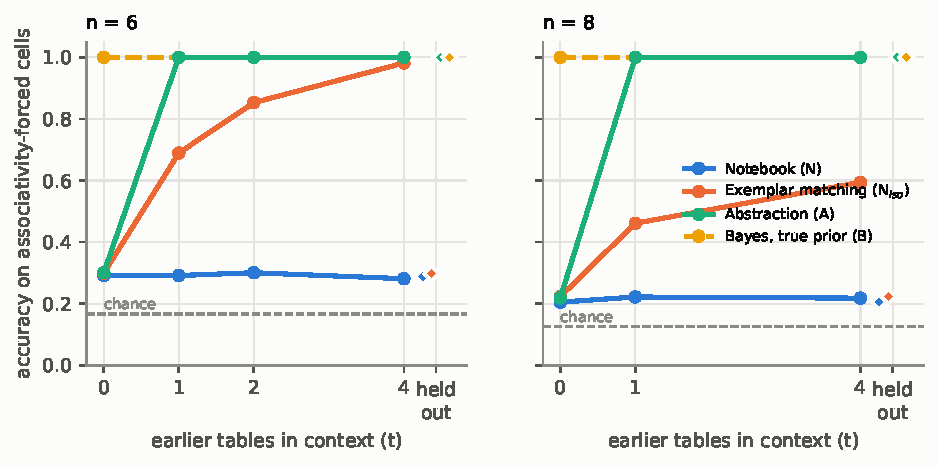
\includegraphics[width=\linewidth,height=0.42\textheight,keepaspectratio]{fig/fig1_ideal_learners.pdf}
\caption{Accuracy of the exact idealised learners on associativity-forced (G) cells against the number of earlier complete tables t, at n=6 (left) and n=8 (right), with held-out types at t=4 shown as diamonds. Abstraction (A) and exemplar matching (N\_iso) both rise with t, but only A transfers to held-out types; the notebook learner (N) stays flat, and Bayes with the true prior (B) is at ceiling from t=0.}\label{fig:ideal}
\end{figure}

\subsection{Pretrained models: class R, and no detectable gain beyond the scramble}\label{sec:r-llm}

All nine checkpoints (ten model--precision configurations) from three families are classified R at both n=6 and n=8, on both accuracy and $p_{\mathrm{gold}}$ (Table~\ref{tab:recall}): accuracy on Latin-forced cells at t=0 ($\mathrm{acc}_L$) is 0.14--0.29, several values are at or below chance (0.167), and every value is below the preregistered threshold of 0.417.

\paragraph{No detectable gain beyond the scramble}

At n=6, t4 $-$ scramble lies between $-$0.019 and +0.026 (Qwen3-8B-Base: $-$0.008 [$-$0.038, +0.022]), and every 95\% CI includes 0 (Figure~\ref{fig:llm}). The largest upper bound, +0.056 (Qwen3-4B-Base), is an order of magnitude below the gains of N\_iso (+0.718) and A (+0.701). Held-out minus scramble lies between $-$0.04 and +0.02. Type-matched (post hoc), held-out minus scramble at $n = 6$ lies between $-$0.038 and +0.012 for the ten configurations, every CI including 0, and having the target's type in the history adds at most +0.033 (every CI including 0), against +0.681 for N\_iso. The one raw held-out contrast that excluded 0, Qwen3-0.6B's $-$0.040 [$-$0.073, $-$0.007] against all scramble trials, is +0.001 [$-$0.037, +0.038] type-matched, so it reflected the difficulty of S3 targets rather than the history.

Two raw increases from t=0 to t=4 have CIs excluding 0, and both are no longer distinguishable from zero against the scramble history: OLMo-2-1B at n=6 gains +0.042 [+0.011, +0.073] from t=0 to t=4 but +0.020 [$-$0.008, +0.051] relative to scramble, and Qwen3-0.6B at n=8 gains +0.031 [+0.014, +0.049] but +0.008 relative to scramble, with a CI that includes 0. OLMo-2-1B's increase (+0.042) also does not survive a post-hoc Bonferroni correction across the 20 model-by-order contrasts (Appendix~\ref{app:mult}); Qwen3-0.6B's at $n = 8$ (+0.031) does. Both raw gains are consistent with effects of context length alone.

\begin{table}[tbp]
\centering
\small
\caption{Pretrained models on the main trials (n=6). Every configuration is class R at n=6 and at n=8. $\mathrm{acc}_L$ is L-cell accuracy at base t=0 (R threshold 0.417); t4 $-$ scr is G accuracy at t=4 minus the scramble history; leak G is G accuracy when the history contains the target's own labelled table. \textsuperscript{\dag} nf4, for which the preregistered quantisation control failed.}\label{tab:recall}
\begin{tabular}{@{}lllll@{}}
\toprule
model & precision & $\mathrm{acc}_L$ & t4 $-$ scr [95\% CI] & leak G \\
\midrule
Qwen3-0.6B & bf16 & 0.289 & $-$0.019 [$-$0.053, +0.014] & 0.620 \\
Qwen3-1.7B & bf16 & 0.193 & +0.012 [$-$0.016, +0.040] & 0.648 \\
Qwen3-0.6B-Base & bf16 & 0.219 & $-$0.003 [$-$0.035, +0.030] & 0.515 \\
Qwen3-1.7B-Base & bf16 & 0.175 & $-$0.007 [$-$0.037, +0.020] & 0.627 \\
Qwen3-1.7B-Base & nf4 \textsuperscript{\dag} & 0.140 & +0.006 [$-$0.022, +0.035] & 0.590 \\
Qwen3-4B-Base & nf4 \textsuperscript{\dag} & 0.202 & +0.026 [$-$0.005, +0.056] & 0.949 \\
Qwen3-8B-Base & nf4 \textsuperscript{\dag} & 0.219 & $-$0.008 [$-$0.038, +0.022] & 0.958 \\
SmolLM2-1.7B & bf16 & 0.184 & +0.002 [$-$0.031, +0.035] & 0.442 \\
OLMo-2-1B & bf16 & 0.228 & +0.020 [$-$0.008, +0.051] & 0.307 \\
OLMo-2-7B & nf4 \textsuperscript{\dag} & 0.158 & $-$0.011 [$-$0.038, +0.017] & 0.365 \\
\bottomrule
\end{tabular}
\end{table}

\paragraph{Recall depends on family more than on size}

When the history contains the target's own labelled table (the leak control), G-cell accuracy is 0.52--0.65 for the Qwen3 models up to 1.7B (0.59 for nf4 Qwen3-1.7B-Base), 0.95 for Qwen3-4B-Base, 0.96 for Qwen3-8B-Base, 0.44 for SmolLM2-1.7B, and 0.31 and 0.37 for OLMo-2-1B and OLMo-2-7B: the larger Qwen3 models retrieve almost perfectly and still stay below the Latin-inference threshold. A post-hoc diagnostic finds a bias towards answering G cells with one of the query's own words, which pulls G accuracy below chance in some models (Appendix~\ref{app:main}).

\begin{figure}[tbp]
\centering
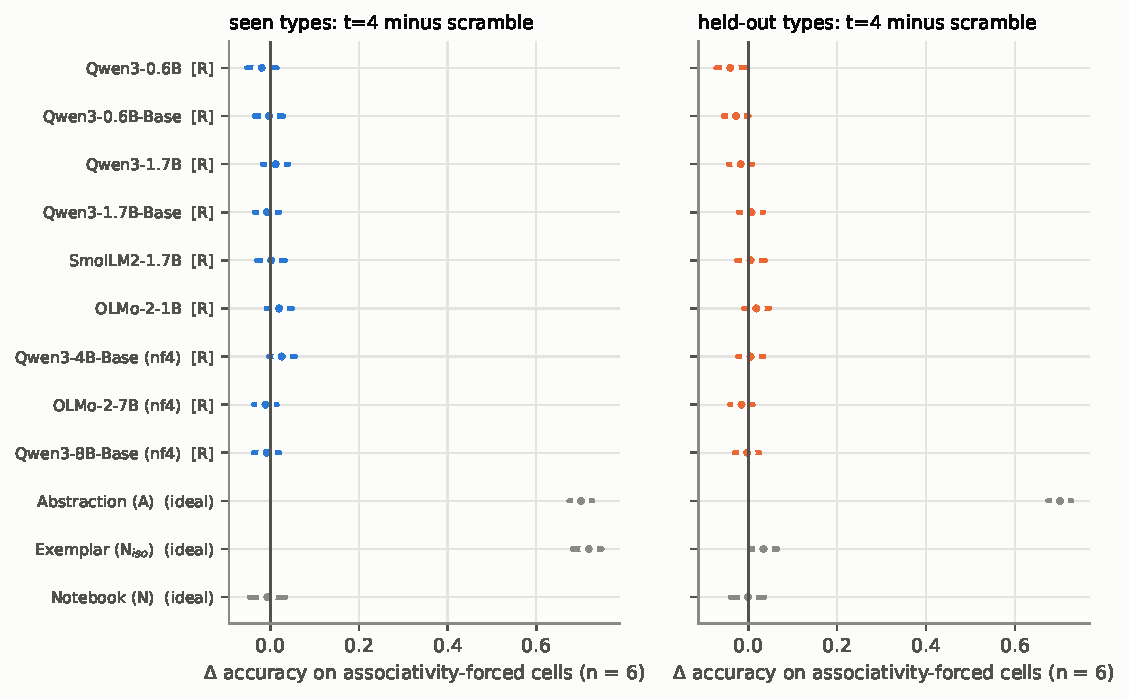
\includegraphics[width=\linewidth,height=0.42\textheight,keepaspectratio]{fig/fig2_llm_contrasts.pdf}
\caption{Compounding contrasts on G cells at n=6: t=4 minus the length-matched scramble history for seen types (left) and for held-out types (right), with 95\% trial-bootstrap CIs, for nine pretrained checkpoints and three idealised learners. Every pretrained interval on seen types includes 0, whereas A and N\_iso sit near +0.70 and only A keeps that gain on held-out types.}\label{fig:llm}
\end{figure}

\subsection{Calibration: Latin accuracy stays near chance up to 8B}\label{sec:r-cal}

On the cue sweep (n=6; k = 10 $\to$ 28 revealed cells of 36), Latin-forced accuracy pooled over t stays close to chance (0.167) for every pretrained model and never comes near the preregistered $k_L$ threshold of 0.5 at any k with at least 30 L queries (Table~\ref{tab:app-cal-k}; Figure~\ref{fig:cal}); only Qwen3-8B-Base (+0.084 [+0.010, +0.153]) and OLMo-2-7B (+0.069 [+0.004, +0.128]) rise marginally from k=10 to k=28. With the guard, $k_L$ is undefined for all eight calibrated models, which are therefore \emph{non-inferential} on this format (the post-trained Qwen3-0.6B was not swept). Without it, Qwen3-0.6B-Base and Qwen3-1.7B-Base qualify at k=6 (2 of 4 L queries correct), which triggers the conditional k=16 step of addendum 2d; run as preregistered after the final audit, it leaves both R ($\mathrm{acc}_L$ 0.177 [0.154, 0.201] and 0.219 [0.196, 0.241]; Appendix~\ref{app:calib}).

\textbf{Missing information does not explain the failure (post hoc).} At k=28, 98\% of the missing cells are Latin-forced (784 of 800), one-pass row/column elimination leaves a single candidate for 86\% of those (675 of 784; \texttt{exp2/\allowbreak{}k28\_elimination.md}), and choosing uniformly among the remaining candidates it would score 0.92 over all missing cells.

Two \emph{exploratory} format variants, row-sorted facts and an instructed header, are reported in Appendix~\ref{app:calib} and summarised in Section~\ref{sec:discussion}. Of the preregistered Experiment-2 hypotheses, H1 is not supported, H2 holds only vacuously and H3 cannot be tested.

\subsection{Trained transformers learn a counting shortcut}\label{sec:r-trained}

The seven networks trained from scratch (Section~\ref{sec:trained}; 3.2M parameters at 4 layers, about 0.91B training tokens each) are all classified R and all fail the recall (leak) control, with leak G accuracy of 0.08--0.24 (Table~\ref{tab:app-main-class}): they neither recall nor infer at sparse cues. In a post-hoc diagnosis, the learned networks answer each trial with essentially one word, the target word least represented among the revealed facts (\texttt{exp3/\allowbreak{}heur/\allowbreak{}}): in A4, 98.6\% of predictions fall in that least-revealed set, which across cells holds about 30\% of the target words. A4's accuracy equals that of the count shortcut C to within 0.001 on all 1,800 main trials ($-$0.0008 [$-$0.0017, +0.0001]) and on the cue sweep, and A1, A2, G4 and I4 match C to within 0.007 (Figure~\ref{fig:trained}); only the 6-layer A6 beats it, by +0.014 [+0.012, +0.015], and P4, which is not learned, does not follow it (Appendix~\ref{app:trained}).

The shortcut also explains the in-training plateau (0.33 at n=6 for the shortcut, 0.29--0.36 for the networks at step 14,000, 0.70 for cell-level row/column elimination) and A4's rise on L cells of the cue sweep (0.17 at k=10 to 0.33 at k=28); over all cells of the sweep, A4's accuracy matches the shortcut's to within 0.004 at every k (Appendix~\ref{app:trained}). The networks therefore learned a global symbol-count statistic, a weak consequence of the Latin property, rather than Latin constraints.

Every run except P4, which memorised its pool without transfer to fresh symbols, exceeds the preregistered learning-failure threshold of chance + 0.10 (0.267) on in-training n=6 remaining-fact accuracy; but the count shortcut alone scores 0.33 (post hoc), so this threshold does not distinguish learning the task from learning the shortcut. Method validation is \emph{not met}: A4 and I4 are R, against predictions of A or B-type and of N\_iso (Table~\ref{tab:trained}), a mismatch that the in-training evaluations, compared post hoc with the count shortcut, attribute to training rather than to the method; the fingerprint gives the networks the same class (R) as the exact count learner C. The preregistered depth prediction is not supported (Appendix~\ref{app:trained}).

\subsection{Positive control: the In-Context Algebra model}\label{sec:r-ica}

\begin{table}[tbp]
\centering
\small
\caption{The released In-Context Algebra model under decision-rule steps 1--3 (base, t=0, accuracy). The R threshold is 1/n + 0.25, and g(G t0) $\geq$ 0.85 would make the model B-type. Every row is classified non-R, non-B, and the class is the same on mean $p_{\mathrm{gold}}$.}\label{tab:ica}
\begin{tabularx}{\linewidth}{@{}>{\raggedright\arraybackslash\hsize=0.6470\hsize}X>{\raggedright\arraybackslash\hsize=1.2941\hsize}X>{\raggedright\arraybackslash\hsize=0.6649\hsize}Xl>{\raggedright\arraybackslash\hsize=1.2941\hsize}X>{\raggedright\arraybackslash\hsize=1.0999\hsize}X@{}}
\toprule
cells & $\mathrm{acc}_L$ [95\% CI] & R threshold & O & G [95\% CI] & g(G t0) [95\% CI] \\
\midrule
n=6, k=10 & 0.886 [0.820, 0.944] & 0.417 & 0.910 & 0.637 [0.601, 0.675] & 0.65 [0.59, 0.74] \\
n=8, k=16 & 0.971 [0.909, 1.000] & 0.375 & 0.988 & 0.663 [0.631, 0.699] & 0.64 [0.58, 0.71] \\
n=5, k=6 & 0.982 [0.952, 1.000] & 0.450 & 0.895 & 0.531 [0.485, 0.574] & 0.42 [0.36, 0.48] \\
n=6, k=16 (2d) & 0.920 [0.900, 0.938] & 0.417 & 0.920 & 0.704 [0.651, 0.758] & 0.71 [0.64, 0.79] \\
\bottomrule
\end{tabularx}
\end{table}

The model is neither R nor B-type (Table~\ref{tab:ica}; Figure~\ref{fig:ica}). At n=6, $\mathrm{acc}_L$ is 0.886 [0.820, 0.944] against a threshold of 0.417 and loop-forced cells score 0.91, while associativity-only (G) cells score 0.637 [0.601, 0.675], so g(G t0) = 0.65 [0.59, 0.74] is below the B-type threshold of 0.85. The same holds at n=8 and n=5, on the addendum-2d k=16 stimuli and on $p_{\mathrm{gold}}$, and O $-$ G is +0.27 to +0.45 in every non-leak cell of the main design that fits the model. This is the first real network for which the fingerprint returns a class above R, and its profile is consistent with its authors' mechanistic analysis: identity, cancellation and copying are near ceiling, and associativity is weakest.

Four of the six preregistered predictions are met (not R; leak recall 1.000; G accuracy above learner C, +0.411 [+0.369, +0.453]; no benefit from a differently labelled history). Two are \emph{not met}: the model is not B-type, and G accuracy is not lower on the order-8 types held out from its training (+0.025 [$-$0.035, +0.085]); accuracy depends more on the specific group than on whether it was seen (Z2$\times$Z2$\times$Z2 and Q8, both unseen, score 0.97 and 0.51; Table~\ref{tab:app-ica-n8}). On the t=0 cue sweep its accuracy over all cells reaches 0.998 at k=28, against 0.29 for Qwen3-8B-Base, 0.33 for learner C and 0.93 for one-pass row/column elimination (Figure~\ref{fig:ica}).

Interleaving all context facts leaves the class unchanged, and across released training checkpoints the class changes from R to non-R between 5k and 10k steps (exploratory; Appendix~\ref{app:ica}). In a post-hoc mechanism split, the model partly answers by commutative copying: when a non-abelian target's transposed cell is revealed but differs from the queried cell, it returns the transpose in 38\% (n=6) to 46\% (n=8) of cases. With the transpose hidden, it beats the exact loop level (Section~\ref{sec:classes}) at n=6 (+0.148 [+0.130, +0.166]) and n=8 (+0.254 [+0.236, +0.273]) but not at n=5 (+0.004 [$-$0.043, +0.048]).

\begin{figure}[tbp]
\centering
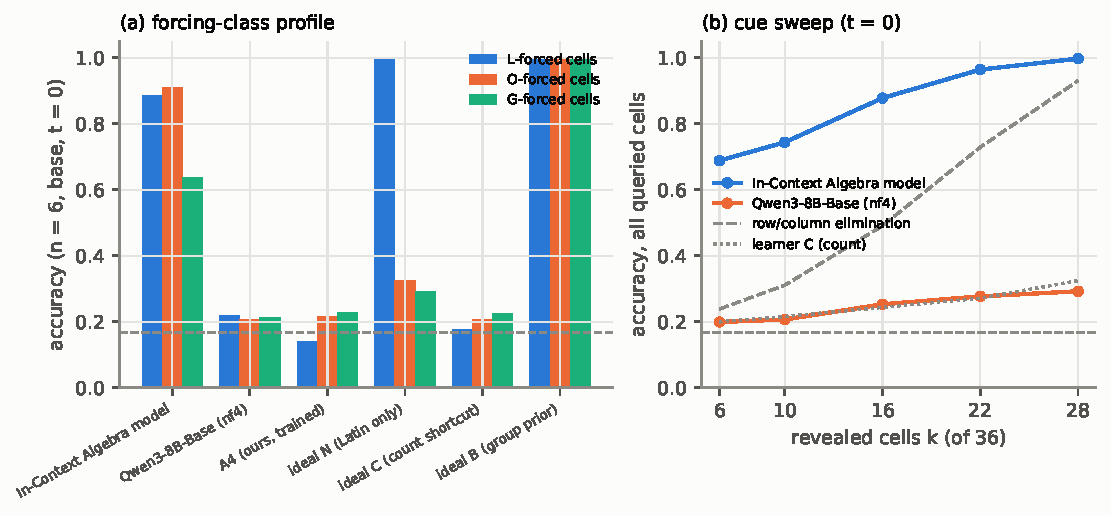
\includegraphics[width=\linewidth,height=0.42\textheight,keepaspectratio]{fig/fig6_in_context_algebra.pdf}
\caption{(a) Accuracy on L-, O- and G-forced cells at n=6, base t=0, for the released In-Context Algebra model, Qwen3-8B-Base, the trained network A4 and the idealised learners N, C and B. (b) Accuracy over all queried cells on the t=0 cue sweep for the In-Context Algebra model and Qwen3-8B-Base, against learner C and one-pass row/column elimination.}\label{fig:ica}
\end{figure}

\subsection{The compute--retrieve axis}\label{sec:r-cr}

Experiment 5 (\emph{preregistered}) tested the compute--retrieve detector of our earlier preprint~\cite{ramdan2026cr} in five Qwen3 models on the leak and base conditions at t=1, which share format, token count and query position but differ in retrievability (accuracy 0.53--0.97 in leak, 0.17--0.22 in base). Its H1, that base projects higher than leak (toward ``compute''), is supported in 0 of 5 models against a criterion of at least 3, and three models are significantly reversed. This holds in the detector's chat-template format; in raw format (exploratory), base significantly exceeds leak in three models. The conditions are not vocabulary-matched: an exploratory control attributes 64--87\% of the reversal to context vocabulary, and with vocabulary matched a retrieval signal of the predicted sign appears in the post-trained model and without the chat template (Appendix~\ref{app:cr}).

\section{Discussion}\label{sec:discussion}

\paragraph{What the study establishes}

Apart from the CR result (Section~\ref{sec:r-cr}), the study establishes four things. First, a measurement, validated on exact learners only, that tells abstraction from exemplar reuse in context: the decision rule recovers all seven preregistered exact learners and the post-hoc count learner C without error, and only held-out transfer cleanly separates abstraction from exemplar matching, also against type-matched baselines (post hoc; Section~\ref{sec:r-ideal}); as the two are provably identical at prime $n$, a claim of ``learning to learn'' an algebraic structure in context needs composite orders and held-out types. Second, an upper bound on history benefit in pretrained language models up to 8B, on this format: none reaches the preregistered Latin-inference threshold in direct-answer mode, and for no model does the 95\% upper bound of the gain from group histories beyond the length-matched scramble exceed +0.056 (+0.069 with a post-hoc Bonferroni correction), an order of magnitude below exemplar copying or abstraction (Section~\ref{sec:r-llm}; Section~\ref{sec:r-cal}). In Qwen3 at 4--8B, which recalls a seen table almost perfectly, the shortfall lies in Latin accuracy (below the preregistered threshold), not in reading the context. Third, a count shortcut that trained networks find instead of the task and that alone passes the preregistered learning-failure threshold, so ``learned'' should be defined against learner C, not chance (Section~\ref{sec:r-trained}). Fourth, a positive control: the In-Context Algebra model~\cite{todd2026ica} is non-R, non-B, with a graded group prior (g(G t0) rises from 0.49 at 10k to 0.65 at 100k training steps; exploratory) that a continuous index captures better than the B-type cut-off (Section~\ref{sec:r-ica}; Table~\ref{tab:app-ica-traj}).

\paragraph{What it does not establish}

We make no claim about larger models, other formats or test-time reasoning. The results are tied to one format, unordered lines of single-token common English words used as arbitrary labels: exploratory row-sorting helps at $k = 28$, most in Qwen3-4B-Base and Qwen3-8B-Base (+0.10 to +0.11) and less (+0.005 to +0.046) elsewhere, including the larger OLMo-2-7B (+0.045), an instruction header does not help ($-$0.08 to +0.04, mean $-$0.006), and grids or natural-language framing may lower the onset scale, although the fingerprint itself is format-independent, because the classes depend only on the cue. An exploratory reasoning probe was dominated by truncation and neither shows nor excludes reasoning-enabled Latin inference (Appendix~\ref{app:probe}).

The method is validated on exact learners only. On trained networks the Experiment-3 validation criterion is \emph{not met} (A4 and I4 are R, not A/B-type and N\_iso) and the depth claim is not supported, which a post-hoc diagnostic attributes to the training rather than to the fingerprint. The In-Context Algebra model is a positive control for steps 1--3 of the rule only, because its 16-token vocabulary rules out the compounding branch.

Nor does Experiment 6 isolate which part of the training matters. The In-Context Algebra model leaves class R after about 0.64--1.28B training tokens, comparable to our roughly 0.91B, but differs in parameters (about 16$\times$ ours), width (1024 vs 256), learning rate, symbol vocabulary (16 vs 64 symbols), loss target (every token vs answers) and context density (groups-only, 200-fact sequences vs sparse cues). Exercising the compounding branch on a trained network needs a model of this kind with enough symbols for $t = 4$ histories (30 at $n = 6$, 40 at $n = 8$), since steps 4 and 5 of the rule use G t4, G scr4 and G held4, and training data in which the count shortcut is uninformative. One data property may matter: the In-Context Algebra generator draws facts with replacement, so, for a guess that ignores the queried cell, symbol counts carry no information about the next answer, whereas our generator writes each table without replacement, which makes the least-revealed symbol the best guess that ignores the cell. Sampling facts with replacement, or reweighting the loss so that least-revealed symbols receive only their uniform share of correct answers, would remove the advantage of this cell-blind shortcut; restricting the loss to cells where the least-revealed symbol is wrong would not, because it rewards the reverse shortcut.

Precision limits the largest models. Qwen3-4B-Base, OLMo-2-7B and Qwen3-8B-Base ran in nf4, whose preregistered control on Qwen3-1.7B-Base failed (G accuracy 0.02--0.07 lower, 44\% of per-query answers changed); it created no spurious effect, but with nothing to hide at 1.7B it cannot rule out that nf4 hides a weak effect at 4B, 7B or 8B, and nf4 accuracies should not be compared with bf16 levels. The CPU-offload path used for OLMo-2-7B and Qwen3-8B-Base was checked against standard scoring only on smaller models, Qwen3-4B-Base in nf4 and Qwen3-1.7B-Base in bf16, not on those two models themselves (Appendix~\ref{app:impl}), and the Qwen3-8B-Base main file, the last 216 trials of the Qwen3-4B-Base main file and the first 50 OLMo-2-7B calibration trials were scored with script versions that were not archived (Appendix~\ref{app:deviations}, row 8).

\paragraph{Threats to validity}

Context length is controlled by a token-matched scramble history for every compounding contrast, and the two raw $t = 0$ to $t = 4$ increases whose CIs exclude 0 (OLMo-2-1B at $n = 6$, Qwen3-0.6B at $n = 8$) are no longer distinguishable from zero against it. Held-out targets are non-abelian only, with abelian histories; the type-matched check leaves every classification and the null unchanged. A held-out arm with non-abelian histories (for example D4 histories with Q8 targets) would also separate exemplar matching from over-generalised commutativity, and remains future work. The main analyses carry no correction for multiple comparisons; a post-hoc Bonferroni correction widens the largest $n = 6$ $t = 4$ minus scramble upper bound from +0.056 to +0.069 and removes OLMo-2-1B's raw increase but not Qwen3-0.6B's (Appendix~\ref{app:mult}).

Freezing the rule and thresholds before any output limits analysis flexibility; the only unplanned change to a decision rule, the $\geq 30$-query guard, excluded a preregistered $k = 16$ follow-up that, once run, leaves both affected models R (Section~\ref{sec:r-cal}). Post-hoc analyses are labelled and enter no preregistered classification; learner C, post hoc in Experiment 3, was fixed before Experiment 6 was preregistered and is its preregistered comparator (prediction P4 in Table~\ref{tab:app-ica-pred}). The scoring checks, the audits and their corrections, none of which changed a fingerprint classification, are described in Appendix~\ref{app:impl}.

\paragraph{Implications}

A model's improvement after seeing related examples is weak evidence of abstraction unless the improvement survives a length-matched control, the cells measured are forced only by the structure in question, and the improvement transfers to held-out types; solving more cells as the cue grows is weak evidence of constraint inference unless it beats a global count baseline. These tests are not blind: on a network trained for the task they return a non-R class and an associativity deficit, consistent with its published mechanisms~\cite{todd2026ica}. The results bound experience compounding at the scale, format and inference mode tested here, rather than exclude it, and give a falsifiable target: sparse-cue Latin inference above the count baseline should precede any compounding, and compounding with $w \approx 1$ should follow.

\section{Conclusion}\label{sec:conclusion}

We built a compounding fingerprint that tells, for partial Cayley tables, whether in-context improvement reflects abstraction or reuse of the examples; its preregistered decision rule recovers seven exact idealised learners without error, but it is so far validated on exact learners only. On this format, none of nine checkpoints (ten model--precision configurations) from three families, up to 8B (4--8B in nf4, whose quantisation control failed), reaches the preregistered Latin-inference threshold in direct-answer mode or gains detectably from group histories beyond a length-matched scramble (every 95\% upper bound at most +0.056); small trained transformers learn a count shortcut; the released In-Context Algebra model is non-R, non-B, inferring Latin- and loop-forced cells almost perfectly but associativity-forced cells only in part; and the compute--retrieve (CR) axis does not track retrieval versus inference on a format- and length-matched (not vocabulary-matched) contrast, where context vocabulary accounts for most of its reversal (exploratory; Appendix~\ref{app:cr}).

Three problems remain open: exercising the compounding branch of the rule on a learned system with enough symbols for $t = 4$ histories, more than the 16-token In-Context Algebra model holds; count-shortcut-aware training, in which ``learned'' is judged against learner C and the data leave the count shortcut uninformative; and matched-vocabulary tests of activation ``mode'' probes before their projections are interpreted.

\section*{Statements}

\paragraph{Preregistration}

Experiments 1, 2, 3, 5 and 6 were preregistered in dated files kept in the repository and frozen before the outputs they govern: 2026-10-06, 2026-10-07, 2026-10-07, 2026-10-08 and 2026-10-11. The exceptions are Experiment 5, whose file was finalised minutes after a discarded six-trial smoke test, and the $\geq 30$-query guard on the Experiment 2 $k_L$ rule, appended after the first calibration sweep had been seen (Appendix~\ref{app:deviations}, row 4). Experiment 4 and Experiment 5b were exploratory designs written down before their final runs: Experiment 4 was redesigned after its first run was truncated, and Experiment 5b followed a 20-trial audit pilot of the same design (Appendix~\ref{app:probe}; Appendix~\ref{app:cr}). Later notes were appended to these files, never edited in. They are not registered with a third party, and the public repository's history starts on 2026-10-12, so the freeze dates rest on the files themselves and on the run logs. Every deviation is listed in Appendix~\ref{app:deviations}.

\paragraph{Audits}

Two adversarial audits (2026-10-07 and 2026-10-09) re-derived every Experiment 1--5 number that existed at the time from the raw result files, using independent code. The results produced after the second audit (learner C, the count-shortcut diagnostic, the offload and re-scoring checks, the full Experiment 5b run and the addendum-2d run) were re-derived instead by later verification passes (2026-10-09), and further passes checked Experiment 6 and the assembled manuscript (2026-10-11). The post-hoc type-matched and multiple-comparisons checks and the worked example of Section~\ref{sec:classes} (2026-10-12) were computed after these passes and were not re-derived by them. The audits used independent code but were run by the same AI system that ran the analyses (see Use of AI assistance), so they are automated self-checks, not independent human review. Each confirmed discrepancy was corrected, and the corrections that changed a reported number or verdict are listed in Appendix~\ref{app:impl} and Appendix~\ref{app:deviations}.

\paragraph{Compute}

All model inference and training used a single laptop GPU (NVIDIA RTX 5070, 8 GB). Exact learners, SAT computations and all analyses ran on the CPU.

\paragraph{Use of AI assistance}

Substantial AI assistance was used throughout this project. An AI system (Claude, Anthropic), working under the author's direction, contributed to the study design, wrote the code and the preregistrations, ran the experiments, analyses and audits, and drafted the text of this paper. The author takes responsibility for the content.

\paragraph{Competing interests}

The author also wrote the compute--retrieve preprint tested in Experiment 5~\cite{ramdan2026cr}. Experiment 5 was preregistered before scoring, its hypothesis and decision rule were fixed in advance, and its result, which does not support the preprint's detector on this contrast, is reported in full. The author declares no other competing interests.

\paragraph{Code and data availability}

Code, stimuli, results and preregistrations are available at \url{https://github.com/Somebodyhere101/compounding-fingerprint}. The repository contains the stimulus generator, the exact forcing-class labels, the idealised learners, the decision rule, all scoring and training scripts, every raw result file, the audit scripts and the preregistrations.

\begin{thebibliography}{99}
\small
\bibitem{xu2020usable} Yilun Xu, Shengjia Zhao, Jiaming Song, Russell Stewart, Stefano Ermon. \newblock A Theory of Usable Information Under Computational Constraints. \newblock International Conference on Learning Representations (ICLR), 2020. \newblock \url{https://arxiv.org/abs/2002.10689}
\bibitem{todd2026ica} Eric Todd, Jannik Brinkmann, Rohit Gandikota, David Bau. \newblock In-Context Algebra. \newblock International Conference on Learning Representations (ICLR), 2026. \newblock \url{https://arxiv.org/abs/2512.16902}
\bibitem{qwen3} An Yang, Anfeng Li, Baosong Yang, et al. \newblock Qwen3 Technical Report. \newblock arXiv:2505.09388, 2025. \newblock \url{https://arxiv.org/abs/2505.09388}
\bibitem{smollm2} Loubna Ben Allal, Anton Lozhkov, Elie Bakouch, et al. \newblock SmolLM2: When Smol Goes Big --- Data-Centric Training of a Fully Open Small Language Model. \newblock Conference on Language Modeling (COLM), 2025. \newblock \url{https://arxiv.org/abs/2502.02737}
\bibitem{olmo2} Team OLMo, Pete Walsh, Luca Soldaini, et al. \newblock 2 OLMo 2 Furious. \newblock Conference on Language Modeling (COLM), shorter version; arXiv:2501.00656, 2025. \newblock \url{https://arxiv.org/abs/2501.00656}
\bibitem{ramdan2026cr} Sam Ramdan. \newblock A Single Direction Separates Computation from Retrieval in Transformer Hidden States. \newblock Zenodo preprint, doi:10.5281/zenodo.19455724; code at github.com/Somebodyhere101/compute-retrieve, 2026. \newblock \url{https://doi.org/10.5281/zenodo.19455724}
\bibitem{notsawo2026grokking} Pascal Jr Tikeng Notsawo, Guillaume Dumas, Guillaume Rabusseau. \newblock Grokking Finite-Dimensional Algebra. \newblock International Conference on Machine Learning (ICML), 2026. \newblock \url{https://arxiv.org/abs/2602.19533}
\bibitem{he2024grok} Tianyu He, Darshil Doshi, Aritra Das, Andrey Gromov. \newblock Learning to grok: Emergence of in-context learning and skill composition in modular arithmetic tasks. \newblock Advances in Neural Information Processing Systems (NeurIPS), 2024. \newblock \url{https://arxiv.org/abs/2406.02550}
\bibitem{huh2025algebraic} Dongsung Huh, Lior Horesh, Halyun Jeong. \newblock A Differentiable Measure of Algebraic Complexity: Provably Exact Discovery of Group Structures. \newblock arXiv:2511.23152, 2025. \newblock \url{https://arxiv.org/abs/2511.23152}
\bibitem{huh2026cayley} Dongsung Huh. \newblock Open Problem: Separating Geometric and Algorithmic Compression via Cayley-Table Completion. \newblock arXiv:2605.29885, 2026. \newblock \url{https://arxiv.org/abs/2605.29885}
\bibitem{raventos2023} Allan Ravent\'os, Mansheej Paul, Feng Chen, Surya Ganguli. \newblock Pretraining task diversity and the emergence of non-Bayesian in-context learning for regression. \newblock Advances in Neural Information Processing Systems (NeurIPS), 2023. \newblock \url{https://arxiv.org/abs/2306.15063}
\bibitem{wurgaft2025} Daniel Wurgaft, Ekdeep Singh Lubana, Core Francisco Park, Hidenori Tanaka, Gautam Reddy, Noah D. Goodman. \newblock In-Context Learning Strategies Emerge Rationally. \newblock Advances in Neural Information Processing Systems (NeurIPS), 2025. \newblock \url{https://arxiv.org/abs/2506.17859}
\bibitem{chan2022} Stephanie C. Y. Chan, Ishita Dasgupta, Junkyung Kim, Dharshan Kumaran, Andrew K. Lampinen, Felix Hill. \newblock Transformers generalize differently from information stored in context vs in weights. \newblock arXiv:2210.05675, 2022. \newblock \url{https://arxiv.org/abs/2210.05675}
\bibitem{xie2021} Sang Michael Xie, Aditi Raghunathan, Percy Liang, Tengyu Ma. \newblock An Explanation of In-context Learning as Implicit Bayesian Inference. \newblock International Conference on Learning Representations (ICLR), 2022. \newblock \url{https://arxiv.org/abs/2111.02080}
\bibitem{olsson2022} Catherine Olsson, Nelson Elhage, Neel Nanda, et al. \newblock In-context Learning and Induction Heads. \newblock Transformer Circuits Thread; arXiv:2209.11895, 2022. \newblock \url{https://arxiv.org/abs/2209.11895}
\bibitem{yang2025symbolic} Yukang Yang, Declan Campbell, Kaixuan Huang, Mengdi Wang, Jonathan Cohen, Taylor Webb. \newblock Emergent Symbolic Mechanisms Support Abstract Reasoning in Large Language Models. \newblock International Conference on Machine Learning (ICML), 2025. \newblock \url{https://arxiv.org/abs/2502.20332}
\bibitem{hendel2023} Roee Hendel, Mor Geva, Amir Globerson. \newblock In-Context Learning Creates Task Vectors. \newblock Findings of EMNLP, 2023. \newblock \url{https://arxiv.org/abs/2310.15916}
\bibitem{todd2023fv} Eric Todd, Millicent L. Li, Arnab Sen Sharma, Aaron Mueller, Byron C. Wallace, David Bau. \newblock Function Vectors in Large Language Models. \newblock International Conference on Learning Representations (ICLR), 2024. \newblock \url{https://arxiv.org/abs/2310.15213}
\bibitem{gurnee2026workspace} Wes Gurnee, Nicholas Sofroniew, Adam Pearce, et al. \newblock Verbalizable Representations Form a Global Workspace in Language Models. \newblock arXiv:2607.15495, 2026. \newblock \url{https://arxiv.org/abs/2607.15495}
\bibitem{wei2023larger} Jerry Wei, Jason Wei, Yi Tay, et al. \newblock Larger language models do in-context learning differently. \newblock arXiv:2303.03846, 2023. \newblock \url{https://arxiv.org/abs/2303.03846}
\bibitem{wu2024reasoning} Zhaofeng Wu, Linlu Qiu, Alexis Ross, et al. \newblock Reasoning or Reciting? Exploring the Capabilities and Limitations of Language Models Through Counterfactual Tasks. \newblock NAACL, 2024. \newblock \url{https://arxiv.org/abs/2307.02477}
\bibitem{gupta2025random} Kavi Gupta, Kate Sanders, Armando Solar-Lezama. \newblock Randomly Sampled Language Reasoning Problems Elucidate Limitations of In-Context Learning. \newblock arXiv:2501.02825, 2025. \newblock \url{https://arxiv.org/abs/2501.02825}
\bibitem{niu2025illusion} Jingcheng Niu, Subhabrata Dutta, Ahmed Elshabrawy, Harish Tayyar Madabushi, Iryna Gurevych. \newblock Illusion or Algorithm? Investigating Memorization, Emergence, and Symbolic Processing in In-Context Learning. \newblock Transactions on Machine Learning Research (TMLR), 2025. \newblock \url{https://arxiv.org/abs/2505.11004}
\bibitem{park2024iclr} Core Francisco Park, Andrew Lee, Ekdeep Singh Lubana, Yongyi Yang, Maya Okawa, Kento Nishi, Martin Wattenberg, Hidenori Tanaka. \newblock ICLR: In-Context Learning of Representations. \newblock International Conference on Learning Representations (ICLR), 2025. \newblock \url{https://arxiv.org/abs/2501.00070}
\bibitem{lepori2026} Michael A. Lepori, Tal Linzen, Ann Yuan, Katja Filippova. \newblock Language Models Struggle to Use Representations Learned In-Context. \newblock Annual Meeting of the Association for Computational Linguistics (ACL), 2026. \newblock \url{https://arxiv.org/abs/2602.04212}
\bibitem{hosseini2026} Eghbal A. Hosseini, Yuxuan Li, Yasaman Bahri, Declan Campbell, Andrew Kyle Lampinen. \newblock Context Structure Reshapes the Representational Geometry of Language Models. \newblock arXiv:2601.22364, 2026. \newblock \url{https://arxiv.org/abs/2601.22364}
\bibitem{matsutani2026} Kohsei Matsutani, Gouki Minegishi, Core Francisco Park, Takeshi Kojima, Yusuke Iwasawa, Yutaka Matsuo. \newblock Few-Shot Demonstrations Elicit the Use of In-Context World Representations in LLMs. \newblock arXiv:2609.24352, 2026. \newblock \url{https://arxiv.org/abs/2609.24352}
\bibitem{hatami2016} Hamed Hatami, Yingjie Qian. \newblock Teaching dimension, VC dimension, and critical sets in Latin squares. \newblock Journal of Combinatorics 9(1), 2018. \newblock \url{https://arxiv.org/abs/1606.00032}
\bibitem{ignatiev2018pysat} Alexey Ignatiev, Antonio Morgado, Joao Marques-Silva. \newblock PySAT: A Python Toolkit for Prototyping with SAT Oracles. \newblock Theory and Applications of Satisfiability Testing (SAT), 2018. \newblock \url{https://pysathq.github.io}
\bibitem{dettmers2023qlora} Tim Dettmers, Artidoro Pagnoni, Ari Holtzman, Luke Zettlemoyer. \newblock QLoRA: Efficient Finetuning of Quantized LLMs. \newblock Advances in Neural Information Processing Systems (NeurIPS), 2023. \newblock \url{https://arxiv.org/abs/2305.14314}
\bibitem{su2021rope} Jianlin Su, Murtadha Ahmed, Yu Lu, Shengfeng Pan, Wen Bo, Yunfeng Liu. \newblock RoFormer: Enhanced Transformer with Rotary Position Embedding. \newblock Neurocomputing 568, 127063, 2024. \newblock \url{https://arxiv.org/abs/2104.09864}
\bibitem{loshchilov2019adamw} Ilya Loshchilov, Frank Hutter. \newblock Decoupled Weight Decay Regularization. \newblock International Conference on Learning Representations (ICLR), 2019. \newblock \url{https://arxiv.org/abs/1711.05101}
\end{thebibliography}
\clearpage
\appendix

\section{Full results for the learners, models and networks}\label{app:main}

Table~\ref{tab:app-main-class} and Table~\ref{tab:app-main-g} give the complete main table: every idealised learner except Asl (which the rule classifies A at $n = 6$ and $n = 8$; Section~\ref{sec:r-ideal}), and every pretrained model and trained network, scored on the identical 1,800 trials. Classes come from the unchanged preregistered decision rule, applied both to accuracy and to mean $p_{\mathrm{gold}}$; the R threshold at $n = 6$ is $\mathrm{acc}_L < 0.417$, and chance on G cells is 0.167. Contrasts carry trial-bootstrap 95\% CIs (2,000 resamples, with seeds fixed per test so that the intervals are reproducible).

Three caveats apply to these tables. First, \textsuperscript{\dag} marks nf4: the preregistered quantisation control failed its tolerance (maximum per-cell G difference 0.067; Appendix~\ref{app:impl}), so absolute G accuracy is biased low by about 0.04 and per-query predictions are unstable, although at 1.7B the class and the t4 $-$ scramble contrast are unchanged. Second, learner C was added post hoc (2026-10-09). Third, for the trained networks class R means only that $\mathrm{acc}_L$ is below threshold: every network also fails the leak control, so it neither recalls nor infers at sparse cues. P4 is \emph{not learned} under the Experiment-3 learning-failure rule and is excluded from method validation.

The preregistered derived quantities comp, held and $w$ are meaningful only above class R, because the rescaling g is undefined when $\mathrm{acc}_L$ is near chance. For the idealised learners at $n = 6$ they separate as designed: N\_iso has comp +0.819 [+0.772, +0.861] and held $-$0.002 [$-$0.043, +0.039] ($w \approx 0$), A has comp and held both +0.839 [+0.802, +0.856] ($w$ = 1.00), and N has comp $-$0.013 [$-$0.064, +0.023]. For every class-R model and network these quantities are uninterpretable, and we do not report them.

\begin{table}[tbp]
\centering
\small
\caption{Class, Latin-forced accuracy and leak-control accuracy for every learner (except Asl), model and network on the identical 1,800 trials. Class is given on accuracy / mean $p_{\mathrm{gold}}$ at $n = 6$ and on accuracy at $n = 8$; $\mathrm{acc}_L$ is at $n = 6$, $t = 0$; leak G is G-cell accuracy in the leak control. \textsuperscript{\dag} nf4.}\label{tab:app-main-class}
\begin{tabularx}{\linewidth}{@{}l>{\raggedright\arraybackslash\hsize=1.5278\hsize}X>{\raggedright\arraybackslash\hsize=0.8856\hsize}X>{\raggedright\arraybackslash\hsize=1.2483\hsize}X>{\raggedright\arraybackslash\hsize=0.6137\hsize}Xl>{\raggedright\arraybackslash\hsize=0.7246\hsize}X@{}}
\toprule
group & learner/model & precision & class n6 (acc / $p_{\mathrm{gold}}$) & class n8 & $\mathrm{acc}_L$ & leak G \\
\midrule
idealised & R (recall) & exact & R / R & R & 0.132 & 1.000 \\
idealised & N (Latin notebook) & exact & N / N & N & 1.000 & 1.000 \\
idealised & N\_iso (exemplar) & exact & N\_iso / N\_iso & N\_iso & 1.000 & 1.000 \\
idealised & A (abstraction) & exact & A / A & A & 1.000 & 1.000 \\
idealised & B (true prior) & exact & B-type / B-type & B-type & 1.000 & 1.000 \\
idealised & Bh (hierarchical) & exact & B-type / B-type & B-type & 1.000 & 1.000 \\
idealised & C (count shortcut; post hoc) & exact & R / R & R & 0.175 & 0.235 \\
pretrained & Qwen3-0.6B & bf16 & R / R & R & 0.289 & 0.620 \\
pretrained & Qwen3-0.6B-Base & bf16 & R / R & R & 0.219 & 0.515 \\
pretrained & OLMo-2-1B & bf16 & R / R & R & 0.228 & 0.307 \\
pretrained & Qwen3-1.7B & bf16 & R / R & R & 0.193 & 0.648 \\
pretrained & Qwen3-1.7B-Base & bf16 & R / R & R & 0.175 & 0.627 \\
pretrained & Qwen3-1.7B-Base & nf4 \textsuperscript{\dag} & R / R & R & 0.140 & 0.590 \\
pretrained & SmolLM2-1.7B & bf16 & R / R & R & 0.184 & 0.442 \\
pretrained & Qwen3-4B-Base & nf4 \textsuperscript{\dag} & R / R & R & 0.202 & 0.949 \\
pretrained & OLMo-2-7B & nf4 \textsuperscript{\dag} & R / R & R & 0.158 & 0.365 \\
pretrained & Qwen3-8B-Base & nf4 \textsuperscript{\dag} & R / R & R & 0.219 & 0.958 \\
trained & A1 & fp32/bf16 & R / R & R & 0.123 & 0.232 \\
trained & A2 & fp32/bf16 & R / R & R & 0.158 & 0.225 \\
trained & A4 & fp32/bf16 & R / R & R & 0.140 & 0.225 \\
trained & A6 & fp32/bf16 & R / R & R & 0.219 & 0.229 \\
trained & G4 & fp32/bf16 & R / R & R & 0.114 & 0.213 \\
trained & P4 & fp32/bf16 & R / R & R & 0.184 & 0.079 \\
trained & I4 & fp32/bf16 & R / R & R & 0.140 & 0.235 \\
\bottomrule
\end{tabularx}
\end{table}

\begin{table}[tbp]
\centering
\small
\caption{G-cell accuracy at $n = 6$ by history condition (base $t = 0$, base $t = 4$, scramble $t = 4$, held-out $t = 4$) and the compounding contrast, base $t = 4$ minus scramble $t = 4$, with its trial-bootstrap 95\% CI. Chance is 0.167. \textsuperscript{\dag} nf4.}\label{tab:app-main-g}
\begin{tabular}{@{}llllll@{}}
\toprule
learner/model & G t0 & G t4 & G scr4 & G held4 & t4 $-$ scr [95\% CI] \\
\midrule
R (recall) & 0.179 & 0.172 & 0.175 & 0.168 & $-$0.004 [$-$0.032, +0.026] \\
N (Latin notebook) & 0.292 & 0.281 & 0.288 & 0.287 & $-$0.007 [$-$0.047, +0.036] \\
N\_iso (exemplar) & 0.299 & 0.981 & 0.263 & 0.298 & +0.718 [+0.682, +0.751] \\
A (abstraction) & 0.301 & 1.000 & 0.299 & 1.000 & +0.701 [+0.675, +0.727] \\
B (true prior) & 1.000 & 1.000 & 1.000 & 1.000 & +0.000 [+0.000, +0.000] \\
Bh (hierarchical) & 1.000 & 1.000 & 0.399 & 1.000 & +0.601 [+0.574, +0.630] \\
C (count shortcut; post hoc) & 0.226 & 0.216 & 0.232 & 0.244 & $-$0.016 [$-$0.041, +0.009] \\
Qwen3-0.6B & 0.150 & 0.160 & 0.179 & 0.139 & $-$0.019 [$-$0.053, +0.014] \\
Qwen3-0.6B-Base & 0.179 & 0.187 & 0.190 & 0.163 & $-$0.003 [$-$0.035, +0.030] \\
OLMo-2-1B & 0.169 & 0.211 & 0.191 & 0.209 & +0.020 [$-$0.008, +0.051] \\
Qwen3-1.7B & 0.115 & 0.120 & 0.108 & 0.091 & +0.012 [$-$0.016, +0.040] \\
Qwen3-1.7B-Base (bf16) & 0.178 & 0.150 & 0.157 & 0.164 & $-$0.007 [$-$0.037, +0.020] \\
Qwen3-1.7B-Base (nf4 \textsuperscript{\dag}) & 0.157 & 0.122 & 0.116 & 0.100 & +0.006 [$-$0.022, +0.035] \\
SmolLM2-1.7B & 0.159 & 0.144 & 0.142 & 0.147 & +0.002 [$-$0.031, +0.035] \\
Qwen3-4B-Base \textsuperscript{\dag} & 0.225 & 0.207 & 0.182 & 0.187 & +0.026 [$-$0.005, +0.056] \\
OLMo-2-7B \textsuperscript{\dag} & 0.173 & 0.166 & 0.176 & 0.161 & $-$0.011 [$-$0.038, +0.017] \\
Qwen3-8B-Base \textsuperscript{\dag} & 0.214 & 0.209 & 0.217 & 0.215 & $-$0.008 [$-$0.038, +0.022] \\
A1 & 0.220 & 0.224 & 0.238 & 0.230 & $-$0.014 [$-$0.037, +0.011] \\
A2 & 0.219 & 0.213 & 0.227 & 0.226 & $-$0.014 [$-$0.037, +0.011] \\
A4 & 0.228 & 0.219 & 0.221 & 0.238 & $-$0.002 [$-$0.026, +0.021] \\
A6 & 0.246 & 0.234 & 0.244 & 0.239 & $-$0.010 [$-$0.036, +0.015] \\
G4 & 0.231 & 0.217 & 0.231 & 0.241 & $-$0.014 [$-$0.037, +0.007] \\
P4 & 0.096 & 0.088 & 0.075 & 0.079 & +0.013 [$-$0.010, +0.036] \\
I4 & 0.241 & 0.215 & 0.228 & 0.239 & $-$0.013 [$-$0.037, +0.009] \\
\bottomrule
\end{tabular}
\end{table}

\paragraph{Exemplar matching at $n = 8$}

At $n = 8$, N\_iso's G accuracy (0.22, 0.46 and 0.59 at $t$ = 0, 1 and 4) tracks the missing mass realised in these stimuli: the target type occurs in the history in 28\% of trials at $t = 1$ and 47\% at $t = 4$. It departs from the design-stage expected-coverage prediction (0.38 and 0.69) because the sampled histories over-cover the target type at $t = 1$ (expected 20\%) and under-cover it at $t = 4$ (expected 59\%).

\paragraph{Answer bias (post hoc)}

A post-hoc diagnostic (\texttt{exp1/\allowbreak{}diag.py}) shows that at $n = 6$ Qwen3-1.7B and SmolLM2-1.7B answer G cells with one of the query's own words in 46\% and 44\% of cases, against 30\% for a uniform guess; over all orders the shares are 39\% and 40\%, against 26\%. Qwen3-0.6B shows no such bias at $n = 6$ (27\% against 30\%) or at $n = 8$ (14\% against 23\%; 19\% against 26\% over all orders). At $n = 5$, however, it too exceeds the uniform rate (46\% against 35\%), and the two 1.7B models score 62\% and 56\%. Because the correct answer is never a query word (0 of 31,553 G cells), this bias pulls G accuracy below chance.

\section{Held-out types against type-matched baselines}\label{app:typematched}

This check is post hoc and was not preregistered. Held-out targets are non-abelian types only (S3 at $n = 6$; D4 or Q8 at $n = 8$), with abelian histories, whereas the base and scramble cells mix target types. We therefore restricted base $t = 0$, base $t = 4$ and scramble $t = 4$ to the trials whose target type is a held-out type (at $n = 6$, 50, 46 and 43 trials; at $n = 8$, 47, 39 and 40) and compared them with the 100 held-out trials of each order, using pooled G-cell accuracy and trial-bootstrap 95\% CIs with 2,000 resamples. Table~\ref{tab:app-typematched} gives the $n = 6$ results: G-cell accuracy on S3 targets at base $t = 0$, scramble $t = 4$ and held-out $t = 4$; held-out minus type-matched scramble; type-matched base $t = 4$ minus held-out, the gain from having the target's type in the history; and, for comparison, the raw held-out contrast against all scramble trials as computed in the main analysis (summarised as a range in Section~\ref{sec:r-llm}).

\begin{table}[tbp]
\centering
\small
\caption{Type-matched held-out check at $n = 6$ (post hoc), with 95\% CIs. \textsuperscript{\dag} nf4; other pretrained models bf16, trained networks fp32/bf16.}\label{tab:app-typematched}
\begin{tabularx}{\linewidth}{@{}>{\raggedright\arraybackslash\hsize=1.4494\hsize}X>{\raggedright\arraybackslash\hsize=0.5303\hsize}X>{\raggedright\arraybackslash\hsize=0.5303\hsize}X>{\raggedright\arraybackslash\hsize=0.5303\hsize}X>{\raggedright\arraybackslash\hsize=1.3199\hsize}X>{\raggedright\arraybackslash\hsize=1.3199\hsize}X>{\raggedright\arraybackslash\hsize=1.3199\hsize}X@{}}
\toprule
learner/model & G t0 & G scr4 & G held4 & held $-$ scr, matched [95\% CI] & t4 $-$ held, matched [95\% CI] & held $-$ scr, all [95\% CI] \\
\midrule
R (recall) & 0.177 & 0.184 & 0.168 & $-$0.016 [$-$0.053, +0.021] & +0.017 [$-$0.019, +0.054] & $-$0.008 [$-$0.037, +0.021] \\
N (Latin notebook) & 0.299 & 0.280 & 0.287 & +0.007 [$-$0.041, +0.057] & +0.008 [$-$0.039, +0.056] & $-$0.000 [$-$0.039, +0.040] \\
N\_iso (exemplar) & 0.307 & 0.264 & 0.298 & +0.033 [$-$0.005, +0.073] & +0.681 [+0.628, +0.721] & +0.034 [$-$0.000, +0.066] \\
A (abstraction) & 0.286 & 0.305 & 1.000 & +0.695 [+0.654, +0.735] & +0.000 [+0.000, +0.000] & +0.701 [+0.675, +0.726] \\
B (true prior) & 1.000 & 1.000 & 1.000 & +0.000 [+0.000, +0.000] & +0.000 [+0.000, +0.000] & +0.000 [+0.000, +0.000] \\
Bh (hierarchical) & 1.000 & 0.458 & 1.000 & +0.542 [+0.504, +0.580] & +0.000 [+0.000, +0.000] & +0.601 [+0.574, +0.630] \\
C (count; post hoc) & 0.215 & 0.243 & 0.244 & +0.000 [$-$0.029, +0.032] & $-$0.025 [$-$0.058, +0.007] & +0.012 [$-$0.014, +0.037] \\
Qwen3-0.6B & 0.147 & 0.138 & 0.139 & +0.001 [$-$0.037, +0.038] & $-$0.005 [$-$0.041, +0.034] & $-$0.040 [$-$0.073, $-$0.007] \\
Qwen3-0.6B-Base & 0.185 & 0.201 & 0.163 & $-$0.038 [$-$0.077, +0.002] & +0.028 [$-$0.014, +0.073] & $-$0.027 [$-$0.056, +0.003] \\
OLMo-2-1B & 0.182 & 0.197 & 0.209 & +0.012 [$-$0.025, +0.048] & +0.001 [$-$0.035, +0.035] & +0.018 [$-$0.012, +0.048] \\
Qwen3-1.7B & 0.109 & 0.090 & 0.091 & +0.001 [$-$0.031, +0.030] & +0.021 [$-$0.010, +0.052] & $-$0.017 [$-$0.046, +0.010] \\
Qwen3-1.7B-Base & 0.174 & 0.172 & 0.164 & $-$0.008 [$-$0.050, +0.029] & $-$0.018 [$-$0.053, +0.016] & +0.007 [$-$0.019, +0.036] \\
Qwen3-1.7B-Base \textsuperscript{\dag} & 0.157 & 0.134 & 0.100 & $-$0.034 [$-$0.072, +0.004] & +0.033 [$-$0.001, +0.069] & $-$0.016 [$-$0.044, +0.011] \\
SmolLM2-1.7B & 0.153 & 0.165 & 0.147 & $-$0.018 [$-$0.068, +0.026] & $-$0.001 [$-$0.036, +0.037] & +0.005 [$-$0.027, +0.037] \\
Qwen3-4B-Base \textsuperscript{\dag} & 0.226 & 0.188 & 0.187 & $-$0.001 [$-$0.031, +0.033] & +0.032 [$-$0.007, +0.069] & +0.005 [$-$0.022, +0.034] \\
OLMo-2-7B \textsuperscript{\dag} & 0.169 & 0.184 & 0.161 & $-$0.023 [$-$0.057, +0.012] & +0.013 [$-$0.019, +0.046] & $-$0.015 [$-$0.040, +0.011] \\
Qwen3-8B-Base \textsuperscript{\dag} & 0.209 & 0.222 & 0.215 & $-$0.007 [$-$0.048, +0.031] & +0.011 [$-$0.023, +0.048] & $-$0.002 [$-$0.031, +0.027] \\
A1 & 0.220 & 0.245 & 0.230 & $-$0.015 [$-$0.045, +0.014] & +0.007 [$-$0.025, +0.039] & $-$0.008 [$-$0.033, +0.017] \\
A2 & 0.228 & 0.238 & 0.226 & $-$0.011 [$-$0.041, +0.018] & $-$0.007 [$-$0.042, +0.027] & $-$0.001 [$-$0.026, +0.025] \\
A4 & 0.231 & 0.236 & 0.238 & +0.003 [$-$0.024, +0.029] & $-$0.010 [$-$0.040, +0.020] & +0.017 [$-$0.004, +0.042] \\
A6 & 0.253 & 0.259 & 0.239 & $-$0.020 [$-$0.047, +0.007] & +0.014 [$-$0.020, +0.046] & $-$0.005 [$-$0.029, +0.020] \\
G4 & 0.233 & 0.243 & 0.241 & $-$0.003 [$-$0.030, +0.023] & $-$0.004 [$-$0.030, +0.024] & +0.009 [$-$0.014, +0.032] \\
P4 & 0.100 & 0.088 & 0.079 & $-$0.009 [$-$0.039, +0.022] & $-$0.001 [$-$0.027, +0.023] & +0.005 [$-$0.019, +0.028] \\
I4 & 0.241 & 0.230 & 0.239 & +0.009 [$-$0.017, +0.036] & $-$0.011 [$-$0.040, +0.018] & +0.010 [$-$0.011, +0.033] \\
\bottomrule
\end{tabularx}
\end{table}

The separation of the idealised learners survives the restriction. A keeps its held-out gain (+0.695 [+0.654, +0.735]); N\_iso's held-out contrast stays small (+0.033 [$-$0.005, +0.073]), and on the same target types it gains +0.681 [+0.628, +0.721] when the target's type is in the history. For every pretrained model, both type-matched contrasts include 0. Qwen3-0.6B's raw held-out contrast, the only one of the ten that excluded 0 ($-$0.040 [$-$0.073, $-$0.007]), is +0.001 [$-$0.037, +0.038] type-matched, so it reflected the difficulty of S3 targets rather than the history.

At $n = 8$ the pattern is the same: held-out minus type-matched scramble is +0.774 [+0.751, +0.797] for A, and N\_iso gains +0.326 [+0.201, +0.453] when the target's type is in the history. For every language model and trained network, the type-matched held-out minus scramble and base $t = 4$ minus held-out contrasts at $n = 8$ include 0, except P4's held-out minus scramble ($-$0.020 [$-$0.036, $-$0.004]).

Held-out histories also move accuracy relative to no history on the same target types in a few configurations. At $n = 6$ they lower S3 accuracy in two nf4 configurations, Qwen3-1.7B-Base (held $-$ t0 $-$0.056 [$-$0.090, $-$0.022]) and Qwen3-4B-Base ($-$0.039 [$-$0.077, $-$0.001]). At $n = 8$, held $-$ t0 excludes 0 for Qwen3-0.6B (+0.021 [+0.004, +0.038]), OLMo-2-1B (+0.027 [+0.008, +0.045]) and OLMo-2-7B ($-$0.019 [$-$0.037, $-$0.003]), and its upper bound rounds to $-$0.000 for Qwen3-1.7B-Base in nf4 ($-$0.019 [$-$0.037, $-$0.000]) and A2 ($-$0.009 [$-$0.017, $-$0.000]). Held-out histories never contain the target's type, so these differences are not transfer of the target's structure; they reflect either non-specific effects of having a history or differences between the trial sets, since the history-blind learner R shows one of the same size at $n = 8$ (held $-$ t0 $-$0.023 [$-$0.043, $-$0.003]).

\section{Multiple comparisons}\label{app:mult}

The main analyses apply no correction for multiple comparisons. This check is post hoc and was not preregistered. It recomputes the raw G-accuracy contrasts of the ten pretrained-model configurations with a trial bootstrap of 20,000 resamples and applies a Bonferroni correction over the 20 model-by-order $t = 4$ minus $t = 0$ contrasts (99.75\% intervals, $p < 0.0025$) and over the 10 $n = 6$ $t = 4$ minus scramble nulls (99.5\% intervals) (Table~\ref{tab:app-mult}). With more resamples, the 95\% intervals can differ in the third decimal from the 2,000-resample intervals of the main text.

\begin{table}[tbp]
\centering
\small
\caption{Multiple-comparisons check for the pretrained models (post hoc; 20,000 resamples): raw $t = 4$ minus $t = 0$ G-accuracy contrasts with 95\% CIs and bootstrap $p$ at $n = 6$ and $n = 8$, and the $n = 6$ $t = 4$ minus scramble contrast with its Bonferroni-adjusted 99.5\% interval. \textsuperscript{\dag} nf4; other models bf16.}\label{tab:app-mult}
\begin{tabularx}{\linewidth}{@{}>{\raggedright\arraybackslash\hsize=0.9491\hsize}X>{\raggedright\arraybackslash\hsize=1.0169\hsize}Xl>{\raggedright\arraybackslash\hsize=1.0170\hsize}Xl>{\raggedright\arraybackslash\hsize=1.0170\hsize}X@{}}
\toprule
model & n=6 t4 $-$ t0 [95\% CI] & p & n=8 t4 $-$ t0 [95\% CI] & p & n=6 t4 $-$ scr [99.5\% CI] \\
\midrule
Qwen3-0.6B & +0.009 [$-$0.021, +0.039] & 0.5435 & +0.031 [+0.014, +0.049] & 0.0003 & $-$0.019 [$-$0.066, +0.029] \\
Qwen3-0.6B-Base & +0.008 [$-$0.026, +0.043] & 0.6332 & +0.006 [$-$0.010, +0.022] & 0.4694 & $-$0.003 [$-$0.050, +0.044] \\
OLMo-2-1B & +0.042 [+0.010, +0.074] & 0.0103 & +0.013 [$-$0.002, +0.027] & 0.0783 & +0.020 [$-$0.022, +0.062] \\
Qwen3-1.7B & +0.005 [$-$0.024, +0.034] & 0.7463 & +0.006 [$-$0.011, +0.023] & 0.4870 & +0.012 [$-$0.029, +0.053] \\
Qwen3-1.7B-Base & $-$0.028 [$-$0.058, +0.002] & 0.0659 & $-$0.005 [$-$0.019, +0.009] & 0.5042 & $-$0.007 [$-$0.050, +0.033] \\
Qwen3-1.7B-Base \textsuperscript{\dag} & $-$0.035 [$-$0.065, $-$0.005] & 0.0202 & $-$0.014 [$-$0.029, +0.001] & 0.0601 & +0.006 [$-$0.036, +0.046] \\
SmolLM2-1.7B & $-$0.016 [$-$0.048, +0.017] & 0.3362 & $-$0.017 [$-$0.032, $-$0.002] & 0.0254 & +0.002 [$-$0.045, +0.048] \\
Qwen3-4B-Base \textsuperscript{\dag} & $-$0.018 [$-$0.049, +0.014] & 0.2759 & $-$0.022 [$-$0.040, $-$0.004] & 0.0180 & +0.026 [$-$0.017, +0.069] \\
OLMo-2-7B \textsuperscript{\dag} & $-$0.007 [$-$0.036, +0.022] & 0.6350 & $-$0.021 [$-$0.035, $-$0.007] & 0.0034 & $-$0.011 [$-$0.048, +0.028] \\
Qwen3-8B-Base \textsuperscript{\dag} & $-$0.004 [$-$0.036, +0.028] & 0.7932 & $-$0.008 [$-$0.022, +0.005] & 0.2253 & $-$0.008 [$-$0.050, +0.035] \\
\bottomrule
\end{tabularx}
\end{table}

Of the 20 $t = 4$ minus $t = 0$ contrasts, 6 have uncorrected $p < 0.05$ (2 increases, 4 decreases). Only Qwen3-0.6B at $n = 8$ (+0.031; 99.75\% interval [+0.006, +0.058]) survives Bonferroni; OLMo-2-1B's +0.042 at $n = 6$ (99.75\% interval [$-$0.008, +0.090]) does not. Every Bonferroni-adjusted interval of the $t = 4$ minus scramble nulls includes 0, and the largest upper bound rises from +0.056 to +0.069 (Qwen3-4B-Base).

\section{Calibration and the addendum-2d operating point}\label{app:calib}

The cue sweep of Experiment 2a used $n = 6$, histories of $t = 0$ and $t = 4$ tables, and cues from $k = 6$ to $k = 28$ revealed cells, with 50 trials per combination of $t$ and $k$. Table~\ref{tab:app-cal-k} gives Latin-forced accuracy by $k$, pooled over $t$, for the eight calibrated language models and for the trained network A4; $k = 6$ is omitted because its 100 trials contain only 4 L queries. Two pretrained models rise marginally from $k = 10$ to $k = 28$, with CIs excluding 0 (Qwen3-8B-Base and OLMo-2-7B), and neither comes near the preregistered 0.5 threshold at any $k$ with at least 30 L queries. For Qwen3-8B-Base the rise appears at both $t = 0$ (0.22 $\to$ 0.29) and $t = 4$ (0.14 $\to$ 0.23), but neither per-$t$ CI excludes 0, and at $k = 28$ accuracy is lower with four history tables than with none (0.23 against 0.29). OLMo-2-7B starts below chance, at 0.12, and its rise is concentrated at $t = 0$. A4 rises more (+0.160), but its accuracy tracks the count shortcut at every $k$ (Appendix~\ref{app:trained}).

\begin{table}[tbp]
\centering
\small
\caption{Latin-forced accuracy by cue size $k$ ($n = 6$, pooled over $t = 0$ and $t = 4$; chance 0.167), with the $k = 28$ minus $k = 10$ difference and its 95\% CI. \textsuperscript{\dag} nf4.}\label{tab:app-cal-k}
\begin{tabular}{@{}llllll@{}}
\toprule
model & k=10 & k=16 & k=22 & k=28 & k28 $-$ k10 [95\% CI] \\
\midrule
Qwen3-0.6B-Base & 0.163 & 0.177 & 0.200 & 0.196 & +0.034 [$-$0.036, +0.102] \\
Qwen3-1.7B & 0.236 & 0.238 & 0.213 & 0.240 & +0.004 [$-$0.089, +0.087] \\
SmolLM2-1.7B & 0.179 & 0.205 & 0.189 & 0.209 & +0.030 [$-$0.041, +0.100] \\
Qwen3-1.7B-Base & 0.171 & 0.194 & 0.208 & 0.213 & +0.042 [$-$0.034, +0.115] \\
Qwen3-4B-Base \textsuperscript{\dag} & 0.228 & 0.194 & 0.211 & 0.207 & $-$0.021 [$-$0.106, +0.062] \\
Qwen3-8B-Base \textsuperscript{\dag} & 0.179 & 0.219 & 0.254 & 0.263 & +0.084 [+0.010, +0.153] \\
OLMo-2-1B & 0.203 & 0.190 & 0.191 & 0.168 & $-$0.035 [$-$0.112, +0.038] \\
OLMo-2-7B \textsuperscript{\dag} & 0.122 & 0.202 & 0.191 & 0.191 & +0.069 [+0.004, +0.128] \\
A4 (trained, 4 layers) & 0.171 & 0.209 & 0.265 & 0.330 & +0.160 [+0.099, +0.217] \\
\bottomrule
\end{tabular}
\end{table}

\begin{figure}[tbp]
\centering
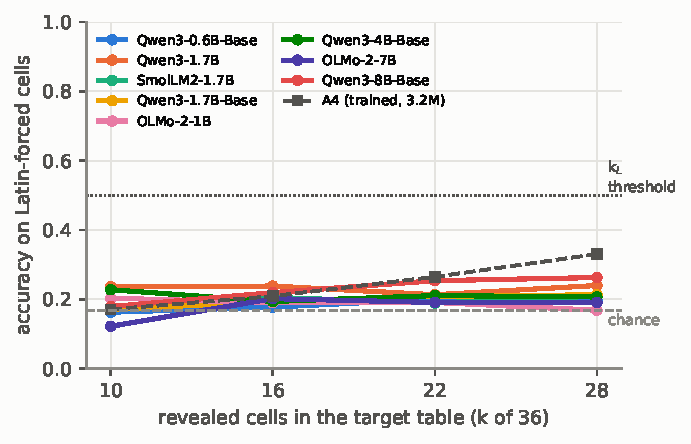
\includegraphics[width=\linewidth,height=0.42\textheight,keepaspectratio]{fig/fig3_calibration.pdf}
\caption{Latin-forced (L) accuracy on the cue sweep (n=6, pooled over t=0 and t=4) against the number of revealed cells k for the eight calibrated pretrained models and the trained network A4, with chance and the preregistered $k_L$ threshold of 0.5 marked. No pretrained model approaches the threshold, and A4's rise follows the count shortcut.}\label{fig:cal}
\end{figure}

\paragraph{The Latin threshold and the conditional $k = 16$ step}

The guard requiring at least 30 pooled L queries per $k$ was added after the Qwen3-0.6B-Base sweep had been seen, because $k = 6$ has only 4 L cells in 100 trials (Appendix~\ref{app:deviations}, row 4). Under the 2a rule as frozen, without the guard, Qwen3-0.6B-Base and Qwen3-1.7B-Base each answer 2 of the 4 L queries at $k = 6$ correctly (0.50), so $k_L = 6$; being R at $k = 10$, they trigger the conditional $k = 16$ operating point of addendum 2d. This is the only adaptive step allowed: it regenerates the $n = 6$ main contrasts at $k = 16$ (100 trials per cell, new seeds) and takes $\mathrm{acc}_L$ from $k = 16$ base $t = 0$. We ran it as specified on 2026-10-09, after the final audit (600 trials per model; chance 0.167, R threshold $\mathrm{acc}_L < 0.417$), and report both readings. Both models remain R, and neither gains beyond the scramble control (Table~\ref{tab:app-cal-2d}). The $\mathrm{acc}_L$ intervals are trial-bootstrap percentile intervals, as computed by the decision rule. With the guard, $k_L$ is undefined for all eight calibrated models.

\begin{table}[tbp]
\centering
\small
\caption{Addendum 2d: the $k = 16$ operating point at $n = 6$ for the two models that the frozen rule sends there. G columns give G-cell accuracy at base $t = 0$, base $t = 4$, and scramble / held-out $t = 4$.}\label{tab:app-cal-2d}
\begin{tabularx}{\linewidth}{@{}>{\raggedright\arraybackslash\hsize=1.4495\hsize}X>{\raggedright\arraybackslash\hsize=1.2657\hsize}X>{\raggedright\arraybackslash\hsize=1.1515\hsize}X>{\raggedright\arraybackslash\hsize=0.5303\hsize}X>{\raggedright\arraybackslash\hsize=0.5303\hsize}X>{\raggedright\arraybackslash\hsize=0.7485\hsize}X>{\raggedright\arraybackslash\hsize=1.3242\hsize}X@{}}
\toprule
model & class (acc / $p_{\mathrm{gold}}$) & $\mathrm{acc}_L$ ($k = 16$, $t = 0$) [95\% CI] & G t0 & G t4 & G scr4 / held4 & t4 $-$ scr [95\% CI] \\
\midrule
Qwen3-0.6B-Base & R / R & 0.177 [0.154, 0.201] & 0.160 & 0.168 & 0.202 / 0.204 & $-$0.034 [$-$0.092, +0.024] \\
Qwen3-1.7B-Base & R / R & 0.219 [0.196, 0.241] & 0.152 & 0.182 & 0.176 / 0.211 & +0.006 [$-$0.058, +0.065] \\
\bottomrule
\end{tabularx}
\end{table}

\paragraph{Format variants (exploratory)}

Neither of the two exploratory variants is used for classification. The sorted variant lists the target's facts grouped by row, at $k \in$ \{16, 22, 28\}; it was added after the first three models swept, all at or below 1.7B (Qwen3-0.6B-Base, Qwen3-1.7B and SmolLM2-1.7B), showed chance-level L accuracy (deviation 5 in Appendix~\ref{app:deviations}). Table~\ref{tab:app-cal-sorted} gives the paired sorted-minus-raw difference on L cells. At $k = 28$ sorting helps Qwen3-4B-Base (+0.108 [+0.066, +0.149]) and Qwen3-8B-Base (+0.101 [+0.061, +0.144]) most, which reach 0.32 and 0.36; it helps Qwen3-1.7B-Base (+0.046), OLMo-2-7B (+0.045) and Qwen3-0.6B-Base (+0.029) less, with CIs excluding 0; it gives similar but non-significant gains for Qwen3-1.7B (+0.027) and SmolLM2-1.7B (+0.024); and it does nothing for OLMo-2-1B (+0.005). Sorted-format gains are therefore not specific to 8B. A4 is unchanged (+0.000), as expected of a count statistic, which ignores fact order.

\begin{table}[tbp]
\centering
\small
\caption{Sorted minus raw accuracy on L cells (exploratory; paired, same trials), with 95\% CIs. \textsuperscript{\dag} nf4.}\label{tab:app-cal-sorted}
\begin{tabularx}{\linewidth}{@{}>{\raggedright\arraybackslash\hsize=0.7593\hsize}X>{\raggedright\arraybackslash\hsize=1.0803\hsize}X>{\raggedright\arraybackslash\hsize=1.0802\hsize}X>{\raggedright\arraybackslash\hsize=1.0802\hsize}X@{}}
\toprule
model & k=16 & k=22 & k=28 \\
\midrule
Qwen3-0.6B-Base & +0.021 [$-$0.005, +0.046] & +0.006 [$-$0.018, +0.029] & +0.029 [+0.001, +0.059] \\
Qwen3-1.7B & $-$0.004 [$-$0.029, +0.022] & +0.029 [+0.005, +0.054] & +0.027 [$-$0.009, +0.061] \\
SmolLM2-1.7B & +0.010 [$-$0.014, +0.033] & +0.017 [$-$0.007, +0.041] & +0.024 [$-$0.010, +0.061] \\
Qwen3-1.7B-Base & +0.015 [$-$0.012, +0.043] & +0.016 [$-$0.010, +0.041] & +0.046 [+0.010, +0.080] \\
Qwen3-4B-Base \textsuperscript{\dag} & +0.022 [$-$0.007, +0.050] & +0.029 [+0.002, +0.055] & +0.108 [+0.066, +0.149] \\
Qwen3-8B-Base \textsuperscript{\dag} & +0.011 [$-$0.014, +0.038] & +0.030 [+0.003, +0.058] & +0.101 [+0.061, +0.144] \\
OLMo-2-1B & $-$0.016 [$-$0.042, +0.008] & +0.002 [$-$0.019, +0.024] & +0.005 [$-$0.018, +0.029] \\
OLMo-2-7B \textsuperscript{\dag} & $-$0.007 [$-$0.032, +0.017] & +0.035 [+0.014, +0.057] & +0.045 [+0.014, +0.075] \\
A4 (trained, 4 layers) & $-$0.005 [$-$0.019, +0.007] & +0.002 [$-$0.003, +0.007] & +0.000 [+0.000, +0.000] \\
\bottomrule
\end{tabularx}
\end{table}

The instructed variant adds a one-paragraph task header, at $k \in$ \{10, 22\}. Table~\ref{tab:app-cal-instr} lists the instructed-minus-raw differences for every cell with at least 30 queries; this guard, added to the $k_L$ rule after the first sweep (deviation 4), is applied here to every class. Over the eight language models, the 32 L and G contrasts (8 models $\times$ $k \in$ \{10, 22\} $\times$ \{L, G\}, pooled over $t$) range from $-$0.083 to +0.042 (mean $-$0.0063, about $-$0.006), and 2 of their CIs exclude 0, both negative. Over all three classes, the 48 contrasts range from $-$0.083 to +0.053 (mean $-$0.0016), and 3 CIs exclude 0.

\begin{table}[tbp]
\centering
\small
\caption{Instructed minus raw accuracy by forcing class (exploratory; paired, pooled over $t$), with 95\% CIs. Queries per cell are the same for every model: at $k = 10$, L 123, O 1,194 and G 1,217; at $k = 22$, L 1,258, O 94 and G 48. \textsuperscript{\dag} nf4.}\label{tab:app-cal-instr}
\begin{tabularx}{\linewidth}{@{}>{\raggedright\arraybackslash\hsize=0.8008\hsize}Xl>{\raggedright\arraybackslash\hsize=1.0664\hsize}X>{\raggedright\arraybackslash\hsize=1.0664\hsize}X>{\raggedright\arraybackslash\hsize=1.0664\hsize}X@{}}
\toprule
model & k & L & O & G \\
\midrule
Qwen3-0.6B-Base & 10 & $-$0.008 [$-$0.038, +0.019] & $-$0.001 [$-$0.015, +0.015] & $-$0.005 [$-$0.022, +0.012] \\
Qwen3-0.6B-Base & 22 & $-$0.006 [$-$0.019, +0.009] & +0.021 [$-$0.041, +0.093] & +0.000 [$-$0.067, +0.059] \\
Qwen3-1.7B & 10 & +0.000 [$-$0.060, +0.065] & +0.005 [$-$0.018, +0.030] & $-$0.030 [$-$0.048, $-$0.011] \\
Qwen3-1.7B & 22 & $-$0.017 [$-$0.033, $-$0.002] & +0.021 [$-$0.068, +0.128] & $-$0.042 [$-$0.136, +0.000] \\
SmolLM2-1.7B & 10 & +0.008 [$-$0.040, +0.056] & $-$0.018 [$-$0.040, +0.003] & +0.016 [$-$0.001, +0.031] \\
SmolLM2-1.7B & 22 & +0.006 [$-$0.010, +0.023] & $-$0.011 [$-$0.095, +0.069] & $-$0.042 [$-$0.100, +0.000] \\
Qwen3-1.7B-Base & 10 & +0.041 [$-$0.007, +0.087] & $-$0.005 [$-$0.026, +0.016] & $-$0.003 [$-$0.021, +0.015] \\
Qwen3-1.7B-Base & 22 & +0.011 [$-$0.006, +0.029] & +0.053 [$-$0.016, +0.131] & +0.042 [+0.000, +0.107] \\
Qwen3-4B-Base \textsuperscript{\dag} & 10 & +0.033 [$-$0.032, +0.097] & +0.023 [+0.004, +0.043] & $-$0.010 [$-$0.027, +0.009] \\
Qwen3-4B-Base \textsuperscript{\dag} & 22 & $-$0.005 [$-$0.022, +0.013] & +0.032 [$-$0.034, +0.087] & $-$0.042 [$-$0.100, +0.000] \\
Qwen3-8B-Base \textsuperscript{\dag} & 10 & $-$0.008 [$-$0.050, +0.034] & +0.002 [$-$0.018, +0.021] & +0.001 [$-$0.018, +0.020] \\
Qwen3-8B-Base \textsuperscript{\dag} & 22 & $-$0.002 [$-$0.020, +0.018] & $-$0.032 [$-$0.109, +0.035] & +0.000 [+0.000, +0.000] \\
OLMo-2-1B & 10 & $-$0.033 [$-$0.079, +0.008] & +0.011 [$-$0.005, +0.027] & $-$0.006 [$-$0.022, +0.011] \\
OLMo-2-1B & 22 & +0.001 [$-$0.017, +0.018] & +0.000 [$-$0.045, +0.039] & $-$0.083 [$-$0.231, +0.036] \\
OLMo-2-7B \textsuperscript{\dag} & 10 & $-$0.016 [$-$0.050, +0.015] & +0.000 [$-$0.021, +0.021] & $-$0.004 [$-$0.022, +0.014] \\
OLMo-2-7B \textsuperscript{\dag} & 22 & +0.002 [$-$0.016, +0.020] & +0.021 [$-$0.025, +0.067] & +0.000 [$-$0.060, +0.065] \\
\bottomrule
\end{tabularx}
\end{table}

\paragraph{Experiment-2 hypotheses}

The preregistered H1, that L accuracy rises with $k$ for every model, is not supported. Its second part, that $k_L$ falls with scale, cannot be tested with the guard; without it, only two of the smallest models have a $k_L$, an artefact of 4 queries. H2, that any compounding appears only in the larger models, holds vacuously, since no model gains beyond the scramble control. H3, that held-out transfer separates A from N\_iso in a model that compounds, cannot be tested.

\section{Trained networks}\label{app:trained}

\paragraph{Architecture and training}

The networks of Experiment 3 are GPT-style decoders (pre-LN, rotary embeddings~\cite{su2021rope}, width 256, 8 heads, 1, 2, 4 or 6 layers; 3.17M parameters at 4 layers) with a 70-token vocabulary. Training ran for 14,000 AdamW steps~\cite{loshchilov2019adamw} ($\beta$ = 0.9/0.95, weight decay 0.1, clipping 1.0, seed 0) of $\lfloor 65536/L \rfloor$ sequences of length L, each step from a single (n, t), with 500 warmup steps and cosine decay to 10\% of a $6 \times 10^{-4}$ peak ($10^{-3}$ for 1--2 layers); t $\in$ 0--4 (t $\leq$ 2 at n=10, so that sequences fit 2,400 tokens). Each network thus saw about 0.91B training tokens (14,000 steps of up to 65,536 tokens). The target table is complete in training and the loss covers every answer token after the sequence's first fact, so the generator's cue size k, uniform in $[\lceil 0.15 n^{2} \rceil, \lfloor 0.45 n^{2} \rfloor]$, does not affect training. Four runs were interrupted by laptop standby or a scheduler change; three were resumed from their last checkpoint and one retrained from scratch, all reaching the preregistered 14,000 steps on a continuous learning-rate schedule (Appendix~\ref{app:deviations}, rows 10--13).

\paragraph{Diets and preregistered criteria}

Training sequences use orders \{4, 5, 6, 7, 8, 10\} and exclude S3, D4 and Q8, with fresh symbols per table and loss on answer tokens only. The mixed-environment diet (A1, A2, A4, A6, by layer count) draws each sequence from groups (0.5), identity-free Latin squares (0.25) or non-associative loops (0.25), so that history is informative about the environment. Three 4-layer controls use groups only (G4), groups from a fixed pool of 32 labelled tables per order (P4), and an exemplar diet of isomorphic-copy tasks and identity-free Latin squares with no group or identity (I4). Predicted classes were frozen before training. The method counts as validated if A4 is A or B-type, I4 is N\_iso, and P4 and A1 are R or N; a run whose in-training remaining-fact accuracy at $n = 6$ never exceeds chance + 0.10 is \emph{not learned} and excluded from validation. Each network was classified by the unchanged decision rule.

We applied the three preregistered Experiment-3 criteria (\texttt{exp3/\allowbreak{}PREREGISTRATION.md}) after the second audit. Table~\ref{tab:trained} compares the predicted classes with the observed ones.

\begin{table}[tbp]
\centering
\small
\caption{Trained networks: preregistered predictions against observed classes (n=6). t4 $-$ scr is G accuracy at t=4 minus the scramble history; held-out G is G accuracy on held-out types at t=4 (chance 0.167). P4 is \emph{not learned} under the preregistered learning-failure rule and is excluded from method validation.}\label{tab:trained}
\begin{tabularx}{\linewidth}{@{}l>{\raggedright\arraybackslash\hsize=1.1221\hsize}X>{\raggedright\arraybackslash\hsize=0.8013\hsize}X>{\raggedright\arraybackslash\hsize=0.7192\hsize}X>{\raggedright\arraybackslash\hsize=1.6729\hsize}X>{\raggedright\arraybackslash\hsize=0.7192\hsize}X>{\raggedright\arraybackslash\hsize=0.9653\hsize}X@{}}
\toprule
run & diet & predicted & observed & t4 $-$ scr [95\% CI] & held-out G & prediction \\
\midrule
A4 & mixed, 4 layers & A (or B-type) & R & $-$0.002 [$-$0.026, +0.021] & 0.238 & not met \\
G4 & groups only & B-type or N & R & $-$0.014 [$-$0.037, +0.007] & 0.241 & not met \\
I4 & isocopy + Latin & N\_iso & R & $-$0.013 [$-$0.037, +0.009] & 0.239 & not met \\
A1 & mixed, 1 layer & R or N & R & $-$0.014 [$-$0.037, +0.011] & 0.230 & met (trivially) \\
A2 & mixed, 2 layers & N-like, O $\gg$ G & R & $-$0.014 [$-$0.037, +0.011] & 0.226 & not met \\
A6 & mixed, 6 layers & $w$ $\geq$ A4's; maybe B-type & R & $-$0.010 [$-$0.036, +0.015] & 0.239 & not met \\
P4 & fixed pool of 32 tables & R or N & R; not learned & +0.013 [$-$0.010, +0.036] & 0.079 & excluded \\
\bottomrule
\end{tabularx}
\end{table}

Two entries need a note. A2 was predicted to be N-like with O $\gg$ G, but at n=6, t=0 its O and G accuracies are 0.21 and 0.22. A6 has $w$ = 0.57, but the value is uninterpretable because its comp is negative ($-$0.22), and A4's $w$ is undefined.

Under the preregistered learning-failure rule, every run except P4 exceeds chance + 0.10 (0.267) on in-training $n = 6$ remaining-fact accuracy, with maxima of 0.33--0.36. P4 never does (maximum 0.183): it memorised its pool (training loss 0.005) without transfer to fresh symbols, so it is \emph{not learned}; we report it but exclude it from method validation. Because the count shortcut alone scores 0.33, this threshold cannot distinguish learning the task from learning the shortcut. P4's in-training value on the isomorphic-copy condition (1.000) is an artefact of pool mode, in which the generator returns memorised pool tables, and it is not used anywhere. Experiment 3's allowed adaptations (a 2$\times$-steps retrain of A4, an M=8 rerun of P4) did not trigger: A4 passed the learning rule, and P4 did not generalise.

Method validation is \emph{not met}: A4 and I4 are R, against predictions of A or B-type and of N\_iso. The preregistration asks that each mismatch be attributed either to the method or to the training diet. The in-training evaluations, compared post hoc with the count shortcut below, attribute it to training, and on the identical trials the fingerprint returns the same class (R) for the networks as for the exact count learner C.

The depth prediction is not supported. Held-out G accuracy at $t = 4$ is 0.230 (A1), 0.226 (A2), 0.238 (A4) and 0.239 (A6). This is not monotone in depth, and the CIs overlap. comp is undefined for A1, A2 and A4, because their $\mathrm{acc}_L$ is below chance; for A6 it is negative, $-$0.22 [$-$3.24, +0.16].

\paragraph{The count-shortcut diagnostic (post hoc)}

The diagnostic is post hoc. For each trial it defines the least-revealed set, the target words with the fewest occurrences as a result among the revealed cue facts, and it records three quantities: the within-trial constancy of the predictions, the share of predictions that fall in the least-revealed set, and the expected accuracy of learner C (uniform over that set) and of one-pass row/column elimination. At $n = 6$ the least-revealed set holds 0.28--0.34 of the target words, which is therefore the share expected from uniform guessing.

Table~\ref{tab:app-trained-count} summarises all raw-format cells for each run, and Figure~\ref{fig:trained} shows the networks' G accuracy beside the exact learners. The learned networks other than A6 put 85--99\% of their predictions in the least-revealed set and match learner C's accuracy to within 0.007; A4 matches it to within 0.001 on both the 1,800 main trials and the 500 cue-sweep trials. A6 is less constant (75\% in the set) and beats C by +0.0135. P4, which is \emph{not learned}, puts 28\% of its predictions in the set, about the uniform rate, and falls 0.048 below C. The two pretrained models we diagnosed do not follow the shortcut: Qwen3-8B-Base and Qwen3-1.7B-Base put 31--42\% of their predictions in the set, and Qwen3-8B-Base exceeds C on the main trials only because those include its near-perfect leak-control cell (0.970).

\begin{table}[tbp]
\centering
\small
\caption{Count-shortcut diagnostic over all raw-format cells (post hoc): share of predictions in the least-revealed set, and model minus learner C accuracy with its 95\% CI.}\label{tab:app-trained-count}
\begin{tabularx}{\linewidth}{@{}>{\raggedright\arraybackslash\hsize=0.8452\hsize}Xl>{\raggedright\arraybackslash\hsize=0.5749\hsize}X>{\raggedright\arraybackslash\hsize=1.5799\hsize}X@{}}
\toprule
run & trials & share in least-revealed set & model $-$ C [95\% CI] \\
\midrule
A1 (main) & 1,800 & 0.849 & $-$0.0065 [$-$0.0080, $-$0.0050] \\
A2 (main) & 1,800 & 0.932 & $-$0.0025 [$-$0.0037, $-$0.0014] \\
A4 (main) & 1,800 & 0.986 & $-$0.0008 [$-$0.0017, +0.0001] \\
A4 (cue sweep) & 500 & 0.990 & $-$0.0009 [$-$0.0017, $-$0.0001] \\
A6 (main) & 1,800 & 0.747 & +0.0135 [+0.0117, +0.0153] \\
G4 (main) & 1,800 & 0.980 & $-$0.0008 [$-$0.0018, +0.0001] \\
I4 (main) & 1,800 & 0.987 & $-$0.0007 [$-$0.0015, +0.0002] \\
P4 (main) & 1,800 & 0.283 & $-$0.0476 [$-$0.0518, $-$0.0432] \\
Qwen3-8B-Base \textsuperscript{\dag} (main) & 1,800 & 0.409 & +0.0393 [+0.0310, +0.0482] \\
Qwen3-8B-Base \textsuperscript{\dag} (cue sweep) & 500 & 0.421 & $-$0.0210 [$-$0.0302, $-$0.0120] \\
Qwen3-1.7B-Base (cue sweep) & 500 & 0.311 & $-$0.0588 [$-$0.0687, $-$0.0492] \\
\bottomrule
\end{tabularx}
\end{table}

\begin{figure}[tbp]
\centering
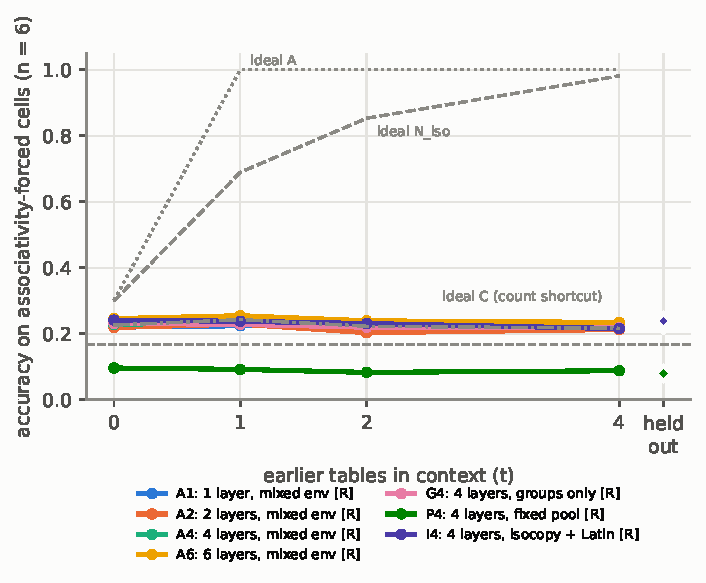
\includegraphics[width=\linewidth,height=0.42\textheight,keepaspectratio]{fig/fig4_trained_transformers.pdf}
\caption{G-cell accuracy (n=6) against the number of earlier tables t for the seven networks trained from scratch, beside the exact learners A, N\_iso and C, with held-out types at t=4 shown at right. Every learned network lies close to the count-shortcut learner C, while P4, which was not learned, sits below chance.}\label{fig:trained}
\end{figure}

Table~\ref{tab:app-trained-sweep} follows A4 across the cue sweep. Its predictions become fully constant within a trial from $k = 16$ on, and its accuracy tracks learner C at every $k$ (within 0.004), rising from 0.196 to 0.334, while row/column elimination would rise from 0.238 to 0.921. On L cells alone, A4 goes from 0.17 at $k = 10$ through 0.21 and 0.26 to 0.33 at $k = 28$ (Table~\ref{tab:app-cal-k}). Qwen3-8B-Base, for comparison, puts 37--48\% of its predictions in the least-revealed set and falls below C at $k = 28$ (0.261 against 0.334).

\begin{table}[tbp]
\centering
\small
\caption{The A4 network across the cue sweep ($n = 6$, 100 trials per $k$, pooled over $t$; post hoc): within-trial constancy, share of predictions in the least-revealed set, and accuracy over all cells for A4, learner C, row/column elimination and Qwen3-8B-Base \textsuperscript{\dag}.}\label{tab:app-trained-sweep}
\begin{tabular}{@{}lllllll@{}}
\toprule
k & A4 constancy & A4 share in set & A4 acc & C acc & row/col acc & Qwen3-8B-Base acc \\
\midrule
6 & 0.92 & 0.95 & 0.196 & 0.200 & 0.238 & 0.194 \\
10 & 0.97 & 0.99 & 0.214 & 0.213 & 0.313 & 0.208 \\
16 & 1.00 & 1.00 & 0.245 & 0.245 & 0.486 & 0.238 \\
22 & 1.00 & 1.00 & 0.272 & 0.274 & 0.715 & 0.260 \\
28 & 1.00 & 1.00 & 0.334 & 0.334 & 0.921 & 0.261 \\
\bottomrule
\end{tabular}
\end{table}

The shortcut also accounts for the in-training plateau. Table~\ref{tab:app-trained-intrain} applies learner C and row/column elimination to the in-training evaluation conditions, teacher-forced and generated with the training generator. Over all remaining facts, the shortcut scores about 0.33 at $n = 6$ and 0.25 at $n = 8$, while elimination would score about 0.70 at $n = 6$. The networks reach 0.29--0.36 at step 14,000. On the identical sequences, averaged over the five evaluation conditions of each order, A4, G4 and I4 sit within $\pm 0.006$ of the shortcut at $n = 6$ and $n = 8$ (single conditions, 64 sequences each, within about $\pm 0.02$), A1 and A2 sit below it, and A6 sits slightly above it (+0.015 at $n = 6$). Their first-fact accuracy after the cue (0.23 for A4 and 0.21 for I4 at step 14,000; chance 0.17) is near the shortcut's level (0.20) and well below elimination (0.30).

\begin{table}[tbp]
\centering
\small
\caption{Expected accuracy of learner C and of one-pass row/column elimination on the in-training evaluation conditions (post hoc; training generator, teacher-forced), over all remaining target facts and on the first fact after the cue.}\label{tab:app-trained-intrain}
\begin{tabularx}{\linewidth}{@{}>{\raggedright\arraybackslash\hsize=2.1264\hsize}Xll>{\raggedright\arraybackslash\hsize=0.7184\hsize}X>{\raggedright\arraybackslash\hsize=0.7184\hsize}X>{\raggedright\arraybackslash\hsize=0.7184\hsize}X>{\raggedright\arraybackslash\hsize=0.7184\hsize}X@{}}
\toprule
condition & n & t & C, all facts & row/col, all facts & C, first fact & row/col, first fact \\
\midrule
in-distribution & 6 & 0 & 0.332 & 0.698 & 0.210 & 0.303 \\
held-out types & 6 & 0 & 0.331 & 0.703 & 0.203 & 0.307 \\
in-distribution & 6 & 4 & 0.334 & 0.705 & 0.192 & 0.290 \\
held-out types & 6 & 4 & 0.327 & 0.710 & 0.198 & 0.283 \\
scramble history & 6 & 4 & 0.331 & 0.710 & 0.181 & 0.306 \\
in-distribution & 8 & 0 & 0.247 & 0.625 & 0.120 & 0.222 \\
held-out types & 8 & 0 & 0.250 & 0.626 & 0.246 & 0.219 \\
in-distribution & 8 & 4 & 0.252 & 0.625 & 0.128 & 0.217 \\
held-out types & 8 & 4 & 0.250 & 0.624 & 0.252 & 0.223 \\
scramble history & 8 & 4 & 0.250 & 0.626 & 0.210 & 0.228 \\
\bottomrule
\end{tabularx}
\end{table}

\section{Reasoning probe (exploratory)}\label{app:probe}

Experiment 4 (\emph{exploratory}, not preregistered) asked whether direct answering limits Latin inference. Qwen3-1.7B answered one Latin-forced cell per trial under a chat prompt stating the Latin-square rule, so the probe measures inference given the rule. Decoding was greedy, with thinking on (at most 4,096 tokens) or off (at most 400); truncated thinking counts as incorrect. The planned design (four conditions $\times$ 30 trials, 1,536 thinking tokens) truncated all 13 thinking answers in its first condition, so we reduced it to 15 trials each of sorted and raw $k = 28$ (Appendix~\ref{app:deviations}, row 17): the first 15 $t = 0$ trials of each format.

With thinking off, the model answered 4 of 15 sorted and 3 of 15 raw trials correctly. With thinking on, it answered 1 of 15 correctly in each format, and 14 of the 15 runs in each format were truncated. In all, 28 of the 30 thinking runs hit the 4,096-token budget. Both runs that finished (2,604 and 3,453 tokens) were correct, but paired by trial, no trial is correct only with thinking on. Six of the 30 non-thinking answers also reached their 400-token limit without an ANSWER line (sorted trials 6 and 8; raw trials 4, 6, 8 and 12). They were scored by the last candidate word mentioned, and all six were incorrect.

The probe is dominated by truncation. It neither shows nor excludes reasoning-enabled Latin inference at this scale, and it tests only whether a model can apply a \emph{stated} rule, not induce one from histories.

\section{The compute--retrieve axis}\label{app:cr}

\paragraph{Background}

A line of activation-space work reads the processing mode from activations. Demonstrations are compressed into a task vector~\cite{hendel2023} or a function vector carried by a few attention heads~\cite{todd2023fv}, and the Jacobian lens identifies representations a model is poised to verbalise, which carry intermediate steps of silent reasoning while automatic processing proceeds without them, as in a global workspace~\cite{gurnee2026workspace}. The compute--retrieve (CR) axis of our earlier preprint~\cite{ramdan2026cr} probes mode directly: a mean-difference direction from 30 retrieval and 30 computation prompts, where ``retrieve'' means recall of facts stored in weights. That preprint notes as a limitation that its retrieval prompts are shorter and less complex than its computation prompts, leaving prompt complexity as a possible confound. Our stimuli remove this confound for in-context retrieval: in the $n = 6$ leak cell at $t = 1$ every query is retrievable, while in base at $t = 1$ the same format, token count and query position require inference. Behaviour differs sharply: accuracy over the queried cells is 0.53--0.97 in leak and 0.17--0.22 in base (0.17--0.21 on the subset of queries projected in Experiment 5).

\paragraph{Design of Experiment 5 (preregistered)}

We ran the published detector code read-only, in bf16 rather than fp16: a mean-difference axis from the paper's 30 + 30 calibration prompts at the best of four layers, read at the last token of chat-template (primary) and raw inputs. The three bf16 models received all 26 queries per trial and the two nf4 models (\textsuperscript{\dag}) 11--12 class-stratified queries, over 100 trials per condition. On Qwen3-0.6B-Base (bf16, uncached forwards) our forward pass reproduced the detector's hidden states exactly; the nf4 and CPU-embedding paths were not checked this way, and the cached path matched uncached forwards in an audit check (r $\geq$ 0.996; Appendix~\ref{app:impl}). H1 predicts that base projects higher, toward ``compute'', than leak; it is supported if the trial-bootstrap CI excludes 0 in that direction in at least 3 of 5 models. H2 predicts a rise in the order L $<$ O $<$ G within base. The hypotheses were finalised minutes after a discarded 6-trial smoke test whose estimate pointed against H1; the direction was kept.

\paragraph{Results of Experiment 5}

The detector separates its own calibration prompts well in every model we tested, with AUC 0.96--0.99 at the chosen layer. Table~\ref{tab:app-cr-h1} reports the preregistered H1 test for each model, together with the exploratory raw-format projection at the same layer. The detector layer is the best of four candidates by calibration AUC. In detector (chat-template) format, base $-$ leak is significantly negative in three models and null in two, so H1 (base $>$ leak, with the CI excluding 0 in at least 3 of 5 models) is supported in 0 of 5. This outcome, a significant reversal, lies outside the preregistered interpretations, which covered only ``supported'' and ``not supported'' (Appendix~\ref{app:deviations}, row 20). In raw format (exploratory), base $>$ leak with the CI excluding 0 in Qwen3-0.6B-Base, Qwen3-1.7B-Base and Qwen3-4B-Base, which would meet the criterion had raw format been primary, and base $<$ leak in Qwen3-1.7B (d = $-$0.28) and Qwen3-8B-Base (d = $-$1.68). H2 (projection rising from L to O to G within base) is null in four models and significantly reversed in Qwen3-1.7B-Base ($\rho$ = $-$0.113 [$-$0.176, $-$0.046]); the other four $\rho$ lie between $-$0.065 and $-$0.003. In an exploratory analysis, projection does not predict correctness within a condition (AUC 0.46--0.55, except 0.38 in Qwen3-1.7B-Base leak).

\begin{table}[tbp]
\centering
\small
\caption{Experiment 5: base minus leak projection on the CR axis at the detector layer, in detector format (preregistered H1) and raw format (exploratory), with trial-bootstrap 95\% CIs, Cohen's d and the query-level AUC for base $>$ leak. Calibration AUC is at the chosen layer. \textsuperscript{\dag} nf4.}\label{tab:app-cr-h1}
\begin{tabularx}{\linewidth}{@{}>{\raggedright\arraybackslash\hsize=1.3297\hsize}X>{\raggedright\arraybackslash\hsize=0.7767\hsize}X>{\raggedright\arraybackslash\hsize=1.5225\hsize}Xl>{\raggedright\arraybackslash\hsize=0.4865\hsize}X>{\raggedright\arraybackslash\hsize=1.3981\hsize}X>{\raggedright\arraybackslash\hsize=0.4865\hsize}X@{}}
\toprule
model & layer (cal. AUC) & detector: base $-$ leak [95\% CI] & d & query AUC & raw: base $-$ leak [95\% CI] & raw d \\
\midrule
Qwen3-0.6B-Base & 26 (0.978) & $-$27.2 [$-$32.7, $-$21.5] & $-$1.34 & 0.19 & +5.8 [+3.8, +7.9] & +0.79 \\
Qwen3-1.7B-Base & 26 (0.964) & $-$158.5 [$-$173.0, $-$144.5] & $-$3.08 & 0.03 & +12.0 [+4.6, +19.6] & +0.44 \\
Qwen3-1.7B & 21 (0.993) & $-$0.06 [$-$1.5, +1.6] & $-$0.01 & 0.50 & $-$1.1 [$-$2.2, $-$0.1] & $-$0.28 \\
Qwen3-4B-Base \textsuperscript{\dag} & 34 (0.973) & $-$11.1 [$-$15.5, $-$6.5] & $-$0.67 & 0.34 & +5.0 [+3.2, +6.7] & +0.77 \\
Qwen3-8B-Base \textsuperscript{\dag} & 34 (0.991) & +0.70 [$-$6.7, +8.0] & +0.03 & 0.51 & $-$24.0 [$-$27.8, $-$20.1] & $-$1.68 \\
\bottomrule
\end{tabularx}
\end{table}

\paragraph{Context vocabulary (Experiment 5b, exploratory)}

Leak and base are matched in format, token count (281 context tokens in both) and query position, but not in vocabulary (Table~\ref{tab:app-cr-surface}). In leak, the history table is written in the target's own six words, so every target line, including the queried pair and its answer, appears verbatim; in base, the history uses six other words. Leak contexts therefore have half the vocabulary, about 5$\times$ more occurrences of the query words, and a verbatim copy of every target line. In detector format the projected token is the template's newline after \texttt{assistant}, so the projection summarises the whole context.

\begin{table}[tbp]
\centering
\small
\caption{Surface statistics of the leak and base contexts.}\label{tab:app-cr-surface}
\begin{tabular}{@{}lll@{}}
\toprule
statistic & leak & base \\
\midrule
distinct content words & 6 & 12 \\
occurrences of the query words in the context & 45.5 & 9.5 \\
repeated 4-gram token fraction & 0.48 & 0.15 \\
query line present verbatim & always & never \\
\bottomrule
\end{tabular}
\end{table}

Experiment 5b (exploratory, not preregistered) followed the H1 result and a 20-trial audit pilot in which relabelling closed 53\% and 71\% of the gap. It was written down before its full run but after that pilot, so it is a full-sample estimate of an effect already seen, not an independent test. It changes only the history table. \textbf{leakRel} permutes the words of leak's history by a random derangement, which keeps its vocabulary but makes its answers inconsistent, so retrievability is the only difference from leak; \textbf{baseRel} writes base's history in the target's words, which keeps it non-retrievable. The share of the target's displayed lines found verbatim in the history is 1.00 for leak, 0.08 for leakRel, 0.11 for baseRel and 0.00 for base. $f_{\mathrm{vocab}} = (\mathrm{baseRel} - \mathrm{base})/(\mathrm{leak} - \mathrm{base})$ is the share of the base--leak gap reproduced by vocabulary alone, and leakRel $-$ leak is the cleanest retrievability contrast (predicted $> 0$). The control used uncached forwards, all 26 queries and 100 trials on four models (8B was not run), so its base $-$ leak values in Table~\ref{tab:app-cr-ctrl} differ slightly from Table~\ref{tab:app-cr-h1}.

\begin{table}[tbp]
\centering
\small
\caption{Experiment 5b vocabulary-overlap control at the detector layer (layer 26 for Qwen3-0.6B-Base and Qwen3-1.7B-Base, 21 for Qwen3-1.7B, 34 for Qwen3-4B-Base \textsuperscript{\dag}), in detector and raw format, with 95\% CIs. $f_{\mathrm{vocab}}$ is uninformative where the base--leak gap is small (Qwen3-1.7B) or where vocabulary moves the projection the other way (Qwen3-1.7B-Base, raw).}\label{tab:app-cr-ctrl}
\begin{tabularx}{\linewidth}{@{}>{\raggedright\arraybackslash\hsize=1.1190\hsize}Xl>{\raggedright\arraybackslash\hsize=0.6280\hsize}X>{\raggedright\arraybackslash\hsize=0.9565\hsize}X>{\raggedright\arraybackslash\hsize=1.3194\hsize}X>{\raggedright\arraybackslash\hsize=0.9771\hsize}X@{}}
\toprule
model & format & base $-$ leak (d) & leak $-$ baseRel [95\% CI] & leakRel $-$ leak [95\% CI] ($d_z$) & $f_{\mathrm{vocab}}$ [95\% CI] \\
\midrule
Qwen3-0.6B-Base & detector & $-$27.26 ($-$1.34) & +8.95 [+3.51, +14.50] & $-$4.36 [$-$6.66, $-$2.05] ($-$0.36) & 0.67 [0.54, 0.85] \\
Qwen3-1.7B-Base & detector & $-$158.59 ($-$3.08) & +20.62 [+5.24, +35.83] & $-$11.83 [$-$20.03, $-$3.52] ($-$0.28) & 0.87 [0.79, 0.96] \\
Qwen3-1.7B & detector & $-$0.07 ($-$0.01) & $-$1.70 [$-$3.07, $-$0.35] & +1.34 [+0.59, +2.07] (+0.36) & 24.72 [$-$35.28, 35.26] \\
Qwen3-4B-Base \textsuperscript{\dag} & detector & $-$10.50 ($-$0.64) & +3.78 [+0.08, +7.36] & $-$1.07 [$-$3.17, +0.95] ($-$0.10) & 0.64 [0.40, 0.99] \\
Qwen3-0.6B-Base & raw & +5.84 (+0.79) & $-$1.88 [$-$4.02, +0.18] & +1.21 [+0.84, +1.61] (+0.60) & 0.68 [0.48, 1.04] \\
Qwen3-1.7B-Base & raw & +12.04 (+0.44) & $-$19.93 [$-$27.49, $-$12.57] & +21.69 [+19.15, +24.19] (+1.67) & $-$0.66 [$-$2.02, $-$0.32] \\
Qwen3-1.7B & raw & $-$1.10 ($-$0.28) & $-$1.10 [$-$2.11, $-$0.03] & +1.75 [+1.26, +2.29] (+0.69) & 1.99 [0.85, 11.49] \\
Qwen3-4B-Base \textsuperscript{\dag} & raw & +4.90 (+0.77) & $-$1.28 [$-$3.05, +0.59] & +0.98 [+0.42, +1.53] (+0.33) & 0.74 [0.53, 1.18] \\
\bottomrule
\end{tabularx}
\end{table}

Vocabulary explains most of the reversal (Figure~\ref{fig:cr}). In the three reversed base models under the chat template, baseRel reproduces 64--87\% of the base--leak gap ($f_{\mathrm{vocab}}$ 0.67 [0.54, 0.85] for Qwen3-0.6B-Base, 0.87 [0.79, 0.96] for Qwen3-1.7B-Base and 0.64 [0.40, 0.99] for Qwen3-4B-Base), and the remainder (leak $-$ baseRel) is still reversed. With vocabulary held fixed (leakRel $-$ leak, predicted $>$ 0), the sign depends on model and wrapper. In detector format the contrast is reversed in Qwen3-0.6B-Base ($d_z$ $-$0.36) and Qwen3-1.7B-Base ($-$0.28), so the retrievable context projects \emph{more} toward compute; it is null in Qwen3-4B-Base ($-$0.10) and in the predicted direction only in the post-trained Qwen3-1.7B (+0.36, and +0.69 in raw format). In raw format at the detector layer it is in the predicted direction in all four models ($d_z$ +0.33 to +1.67), although at other layers the sign varies.

The post-trained null is a cancellation. In Qwen3-1.7B, vocabulary overlap raises the projection (baseRel $-$ base = +1.8) about as much as retrievability lowers it (leak $-$ leakRel = $-$1.3), which is why the preregistered contrast is null there.

The axis therefore carries an in-context retrieval signal of the predicted sign in two places. In the post-trained model it is small ($d_z$ +0.36 in detector format), about the size of that model's vocabulary effect. In raw format it ranges from $d_z$ +0.33 to +1.67, and in Qwen3-1.7B-Base it exceeds the vocabulary effect. In the base models under the detector's chat template, by contrast, the vocabulary effect (baseRel $-$ base) is 4--12$\times$ the retrievability contrast, and with vocabulary held fixed the retrievability contrast itself is reversed in Qwen3-0.6B-Base and Qwen3-1.7B-Base and null in Qwen3-4B-Base.

\begin{figure}[tbp]
\centering
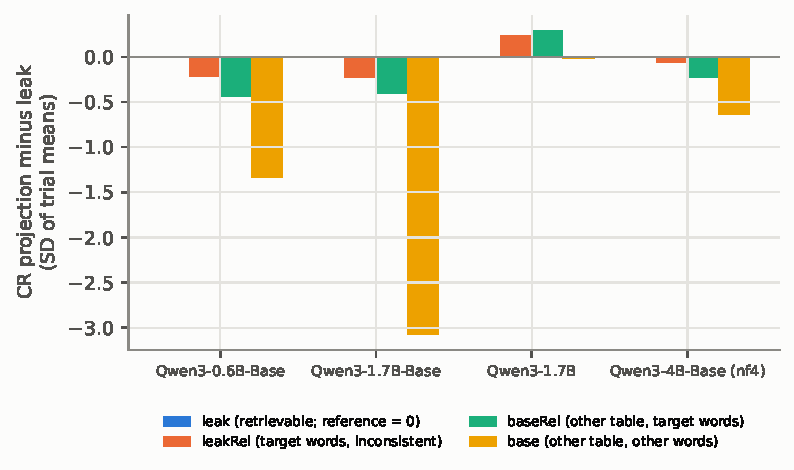
\includegraphics[width=\linewidth,height=0.42\textheight,keepaspectratio]{fig/fig5_cr_axis_control.pdf}
\caption{Experiment 5b (exploratory): CR projection for each condition minus leak, in units of the pooled SD of the leak and base trial means, at the detector layer and in detector (chat-template) format, for four Qwen3 models (8B was not run). Writing a non-retrievable history in the target's words (baseRel) reproduces most of the base--leak gap, and making the retrievable history inconsistent (leakRel) lowers the projection in Qwen3-0.6B-Base and Qwen3-1.7B-Base, against the prediction, has no reliable effect in Qwen3-4B-Base, and raises it, as predicted, only in the post-trained Qwen3-1.7B.}\label{fig:cr}
\end{figure}

\paragraph{Interpretation}

The CR axis separates its calibration prompts with AUC 0.96--0.99, but it does not track retrieval versus inference once format and length are matched: it is significantly reversed in three of five models, and its sign flips with prompt format. An exploratory control attributes 64--87\% of the reversed gap to context vocabulary. With vocabulary matched, a retrieval signal of the predicted sign appears in the post-trained model (small, $d_z$ +0.36, comparable to its vocabulary effect) and without the chat template ($d_z$ +0.33 to +1.67). For representation-level claims about ``modes'' of processing, this is a cautionary case: a direction that separates prompt \emph{types} need not track the \emph{process}. A format- and length-matched behavioural contrast, like leak versus base, is a cheap test that any such probe should pass before it is interpreted, and vocabulary must be matched as well. Whether activation-space representations of processing mode would carry induced axioms across tables is untested.

\section{In-Context Algebra positive control}\label{app:ica}

We re-implemented the released model from its code without executing that code, and loaded the checkpoint with \texttt{weights\_only=True}. A second, independent forward pass (explicit causal attention, real-valued RoPE, erf-GELU) agrees with the adapter on 3,200 of 3,200 answer positions, with a maximum absolute logit difference of $1.9 \times 10^{-4}$. Table~\ref{tab:app-ica-valid} gives held-out final-fact accuracy on the model's own task. Under the upstream evaluation protocol on 1,024 fresh sequences, the released best checkpoint scores 0.959, below the 99.4\% that its authors report~\cite{todd2026ica}. Their figure is the maximum over up to about 290 training-time evaluations on one cached 512-sequence set, and \texttt{algebra\_gpt\_best.pt} was saved at that maximum; the 20k--100k checkpoints score 0.960--0.975 on our sequences, so every released checkpoint from 20k steps on, the best one included, scores 0.959--0.975. The shortfall is therefore consistent with snapshot selection on a fixed set, not with a port error. Full-sequence training loss is 0.917, against about 0.93 at the end of the upstream curve.

\begin{table}[tbp]
\centering
\small
\caption{Validation of the adapter on the model's own distribution: held-out final-fact accuracy.}\label{tab:app-ica-valid}
\begin{tabular}{@{}ll@{}}
\toprule
setting & accuracy \\
\midrule
shuffled vocabulary, 200 facts (512 sequences) & 0.973 \\
shuffled vocabulary, 100 / 50 / 20 facts & 0.91 / 0.83 / 0.66 \\
upstream protocol, 1,024 fresh sequences, best checkpoint & 0.959 \\
same sequences, checkpoints 100k / 40k / 20k / 10k & 0.960 / 0.975 / 0.971 / 0.835 \\
\bottomrule
\end{tabular}
\end{table}

The adapter maps each trial's words to distinct random symbols (four draws; no group identity maps to `0', as in training) and scores each query by forced choice over the target's $n$ symbols; only cells with at most 16 distinct words fit. Decision-rule steps 1--3 need only the base $t = 0$ cell; steps 4--5 need $t = 4$ and scramble histories, which do not fit the 16-token vocabulary. Table~\ref{tab:app-ica-steps} gives these steps for every order, on accuracy and on mean $p_{\mathrm{gold}}$ (stimulus fact order, four symbol draws, bootstrap seeded as in the main analysis). Every row is non-R and non-B, with N, N\_iso and A undetermined. Loop-forced cells score 0.90 ($n = 5$), 0.91 ($n = 6$) and 0.99 ($n = 8$), and O $-$ G is +0.27 to +0.45 in every non-leak cell of the main design that fits the model (base $t = 0$ at $n = 5$, 6 and 8; base and held-out $t = 1$ at $n = 6$ and 8). The addendum-2d $k = 16$ cells keep O above G with a smaller gap (+0.20 to +0.22), with L/O/G accuracy 0.930/0.920/0.710 (base $t = 1$) and 0.909/0.917/0.713 (held-out $t = 1$), and the leak control scores 1.000 on every forcing class.

\begin{table}[tbp]
\centering
\small
\caption{In-Context Algebra model, decision-rule steps 1--3 at base $t = 0$ (preregistered at $n = 6$, primary, and $n = 8$, secondary; the $n = 5$ and addendum-2d rows apply the same steps to the other base $t = 0$ cells that fit the vocabulary), with trial-bootstrap 95\% CIs and the number of L queries. Every row is classified non-R, non-B.}\label{tab:app-ica-steps}
\begin{tabularx}{\linewidth}{@{}>{\raggedright\arraybackslash\hsize=0.6801\hsize}Xl>{\raggedright\arraybackslash\hsize=1.4878\hsize}X>{\raggedright\arraybackslash\hsize=0.7350\hsize}X>{\raggedright\arraybackslash\hsize=1.1336\hsize}X>{\raggedright\arraybackslash\hsize=0.9635\hsize}X@{}}
\toprule
order and cue & measure & $\mathrm{acc}_L$ [95\% CI] (L queries) & R threshold & G t0 [95\% CI] & g(G t0) [95\% CI] \\
\midrule
n=6, k=10 & accuracy & 0.886 [0.820, 0.944] (114) & 0.417 & 0.637 [0.601, 0.675] & 0.65 [0.59, 0.74] \\
n=6, k=10 & $p_{\mathrm{gold}}$ & 0.852 [0.800, 0.897] (114) & 0.417 & 0.541 [0.519, 0.562] & 0.55 [0.50, 0.60] \\
n=8, k=16 & accuracy & 0.971 [0.909, 1.000] (34) & 0.375 & 0.663 [0.631, 0.699] & 0.64 [0.58, 0.71] \\
n=8, k=16 & $p_{\mathrm{gold}}$ & 0.864 [0.804, 0.922] (34) & 0.375 & 0.495 [0.479, 0.513] & 0.50 [0.46, 0.55] \\
n=5, k=6 & accuracy & 0.982 [0.952, 1.000] (111) & 0.450 & 0.531 [0.485, 0.574] & 0.42 [0.36, 0.48] \\
n=5, k=6 & $p_{\mathrm{gold}}$ & 0.901 [0.874, 0.928] (111) & 0.450 & 0.519 [0.496, 0.544] & 0.46 [0.42, 0.50] \\
n=6, k=16 (2d stimuli) & accuracy & 0.920 [0.900, 0.938] (1,106) & 0.417 & 0.704 [0.651, 0.758] & 0.71 [0.64, 0.79] \\
n=6, k=16 (2d stimuli) & $p_{\mathrm{gold}}$ & 0.903 [0.889, 0.917] (1,106) & 0.417 & 0.642 [0.604, 0.680] & 0.64 [0.59, 0.70] \\
\bottomrule
\end{tabularx}
\end{table}

Table~\ref{tab:app-ica-pred} lists the six preregistered predictions. Four are met; two, B-type and lower G accuracy on unseen types, are \emph{not met} and are reported as such.

\begin{table}[tbp]
\centering
\small
\caption{Preregistered predictions for the In-Context Algebra model and their outcomes.}\label{tab:app-ica-pred}
\begin{tabularx}{\linewidth}{@{}>{\raggedright\arraybackslash\hsize=1.4307\hsize}X>{\raggedright\arraybackslash\hsize=0.2730\hsize}X>{\raggedright\arraybackslash\hsize=1.2963\hsize}X@{}}
\toprule
prediction & outcome & evidence \\
\midrule
P1: not R at n=6 & met & $\mathrm{acc}_L$ 0.886 [0.820, 0.944] \\
P2: B-type at n=6 & not met & g(G t0) 0.65, below 0.85: non-R, non-B \\
P3: leak recall, G at least 0.90 & met & leak G 1.000 \\
P4: G above learner C (paired) & met & +0.411 [+0.369, +0.453] \\
P5: no gain from a differently labelled history (n=6 G, t1 $-$ t0) & met & $-$0.025 [$-$0.071, +0.024] \\
P6: unseen order-8 types below seen types (n8 base t0) & not met & +0.025 [$-$0.035, +0.085]; pooled n=8 cells $-$0.005 [$-$0.036, +0.026] \\
\bottomrule
\end{tabularx}
\end{table}

Table~\ref{tab:app-ica-n8} breaks $n = 8$ G accuracy down by target type. Z8 (= C8) and D4 were in the model's training mix; Z4$\times$Z2, Z2$\times$Z2$\times$Z2 and Q8 were not. G accuracy depends on the specific group more than on whether it was seen: at base $t = 0$, Z2$\times$Z2$\times$Z2, whose smaller relative Z2$\times$Z2 (= D2) was in training, scores 0.973, and Q8 scores 0.507. Latin- and loop-forced accuracy is 0.95--1.00 for seen and unseen types alike.

\begin{table}[tbp]
\centering
\small
\caption{G-cell accuracy at $n = 8$ by target type (seen in training: Z8, D4), with pooled seen / unseen accuracy.}\label{tab:app-ica-n8}
\begin{tabular}{@{}lllllll@{}}
\toprule
cell & Z8 & D4 & Z4$\times$Z2 & Z2$\times$Z2$\times$Z2 & Q8 & seen / unseen \\
\midrule
base t0 & 0.627 & 0.671 & 0.673 & 0.973 & 0.507 & 0.648 / 0.673 \\
base t1 & 0.544 & 0.601 & 0.619 & 0.773 & 0.458 & 0.562 / 0.601 \\
held-out t1 & --- & 0.575 & --- & --- & 0.464 & 0.575 / 0.464 \\
\bottomrule
\end{tabular}
\end{table}

At $n = 6$, base $t = 0$, the model scores 0.886 (L), 0.910 (O) and 0.637 (G), against 0.148, 0.212 and 0.226 for learner C and 0.563, 0.314 and 0.289 for one-pass row/column elimination; it beats both baselines by a wide margin in every class. Table~\ref{tab:app-ica-sweep} places its cue sweep next to Qwen3-8B-Base, learner C and elimination on the same $t = 0$ trials. Row-sorting the facts makes no difference for this model (0.881 against 0.878 at $k = 16$). Interleaving all context facts in one random order (exploratory) also changes nothing: at $n = 6$, base $t = 0$, L, O and G score 0.886, 0.908 and 0.647, and the class is the same at $n = 5$, 6 and 8.

\begin{table}[tbp]
\centering
\small
\caption{Cue sweep at $n = 6$, $t = 0$: accuracy over all queried cells for the In-Context Algebra model and Qwen3-8B-Base \textsuperscript{\dag} (raw and row-sorted facts), and the expected accuracy of learner C and one-pass row/column elimination on the same trials.}\label{tab:app-ica-sweep}
\begin{tabularx}{\linewidth}{@{}l>{\raggedright\arraybackslash\hsize=0.9492\hsize}X>{\raggedright\arraybackslash\hsize=0.7593\hsize}X>{\raggedright\arraybackslash\hsize=0.9492\hsize}X>{\raggedright\arraybackslash\hsize=0.9523\hsize}X>{\raggedright\arraybackslash\hsize=1.1950\hsize}X>{\raggedright\arraybackslash\hsize=1.1950\hsize}X@{}}
\toprule
k & model, raw & model, sorted & learner C & row/col elimination & Qwen3-8B-Base, raw & Qwen3-8B-Base, sorted \\
\midrule
6 & 0.689 & --- & 0.200 & 0.239 & 0.199 & --- \\
10 & 0.744 & --- & 0.216 & 0.311 & 0.207 & --- \\
16 & 0.878 & 0.881 & 0.244 & 0.491 & 0.253 & 0.264 \\
22 & 0.964 & 0.964 & 0.271 & 0.729 & 0.277 & 0.289 \\
28 & 0.998 & 0.998 & 0.325 & 0.931 & 0.292 & 0.407 \\
\bottomrule
\end{tabularx}
\end{table}

Table~\ref{tab:app-ica-traj} follows six of the 21 released numbered checkpoints (exploratory; $n = 6$, base $t = 0$, two symbol draws). The checkpoints at 0 and 5k steps are R, and those from 10k on are non-R, non-B; the upstream training loss drops sharply between those steps. After 20k, Latin and loop accuracy plateau at 0.86--0.91 while g(G t0) keeps rising, a graded change that a continuous index captures and the categorical classes do not.

\begin{table}[tbp]
\centering
\small
\caption{Training trajectory of the In-Context Algebra model across released checkpoints (exploratory), with the class from decision-rule steps 1--3 and cue-sweep accuracy at $k = 28$.}\label{tab:app-ica-traj}
\begin{tabular}{@{}lllllll@{}}
\toprule
step & $\mathrm{acc}_L$ & O t0 & G t0 & g(G t0) & class & sweep k=28 \\
\midrule
0 & 0.167 & 0.155 & 0.162 & --- & R & 0.172 \\
5k & 0.351 & 0.392 & 0.250 & 0.45 & R & 0.575 \\
10k & 0.807 & 0.840 & 0.483 & 0.49 & non-R, non-B & 0.930 \\
20k & 0.860 & 0.885 & 0.550 & 0.55 & non-R, non-B & 0.988 \\
40k & 0.868 & 0.896 & 0.600 & 0.62 & non-R, non-B & 0.988 \\
100k & 0.886 & 0.911 & 0.635 & 0.65 & non-R, non-B & 0.998 \\
\bottomrule
\end{tabular}
\end{table}

The mechanism split is post hoc, added after the primary results. It pools the base $t = 0$ and $t = 1$ and held-out $t = 1$ cells of each order, and it splits G cells by whether the target is abelian and whether the transposed cell $b \cdot a$ is revealed in the cue. The baselines are expected accuracies on the same cells: learner N (uniform over Latin-feasible values), an exact loop-level learner (uniform over the values that a loop completion of the cue allows, computed with the stimulus generator's SAT engine) and learner C. G cells are by definition not loop-forced, so beating the loop-level learner requires group structure beyond identity and cancellation (Table~\ref{tab:app-ica-mech}).

\begin{table}[tbp]
\centering
\small
\caption{Mechanism split of G cells (post hoc), pooled over the base $t = 0$/$t = 1$ and held-out $t = 1$ cells of each order: model accuracy (number of cells), share of predictions equal to the revealed transpose, and the expected accuracy of the loop-level learner and of learners N and C.}\label{tab:app-ica-mech}
\begin{tabularx}{\linewidth}{@{}ll>{\raggedright\arraybackslash\hsize=1.2278\hsize}X>{\raggedright\arraybackslash\hsize=1.1437\hsize}X>{\raggedright\arraybackslash\hsize=0.8120\hsize}X>{\raggedright\arraybackslash\hsize=0.5046\hsize}X>{\raggedright\arraybackslash\hsize=1.3119\hsize}X@{}}
\toprule
order & target & transpose & G acc (cells) & pred. = transpose & loop level & N / C \\
\midrule
n=5 & abelian & hidden & 0.460 (463) & 0.000 & 0.456 & 0.322 / 0.290 \\
n=5 & abelian & revealed, = gold & 1.000 (70) & 1.000 & 0.474 & 0.304 / 0.029 \\
n=6 & abelian & hidden & 0.628 (872) & 0.000 & 0.430 & 0.300 / 0.272 \\
n=6 & abelian & revealed, = gold & 0.963 (214) & 0.963 & 0.415 & 0.281 / 0.063 \\
n=6 & non-abelian & hidden & 0.542 (1,947) & 0.000 & 0.417 & 0.301 / 0.239 \\
n=6 & non-abelian & revealed, $\neq$ gold & 0.583 (504) & 0.377 & 0.427 & 0.285 / 0.248 \\
n=6 & non-abelian & revealed, = gold & 1.000 (60) & 1.000 & 0.417 & 0.295 / 0.057 \\
n=8 & abelian & hidden & 0.610 (3,206) & 0.000 & 0.292 & 0.221 / 0.194 \\
n=8 & abelian & revealed, = gold & 0.925 (859) & 0.925 & 0.286 & 0.212 / 0.032 \\
n=8 & non-abelian & hidden & 0.501 (4,918) & 0.000 & 0.289 & 0.220 / 0.171 \\
n=8 & non-abelian & revealed, $\neq$ gold & 0.425 (760) & 0.458 & 0.290 & 0.216 / 0.168 \\
n=8 & non-abelian & revealed, = gold & 0.943 (601) & 0.943 & 0.283 & 0.215 / 0.038 \\
\bottomrule
\end{tabularx}
\end{table}

Two mechanisms are visible. When a non-abelian target's transpose is revealed but differs from the queried cell, the model copies it 38\% ($n = 6$) or 46\% ($n = 8$) of the time, a commutativity shortcut that fails on non-abelian groups. With the transpose hidden, the model beats the loop-level learner at $n = 6$ (+0.148 [+0.130, +0.166]; 282 trials, 2,819 cells) and at $n = 8$ (+0.254 [+0.236, +0.273]; 300 trials, 8,124 cells), but not at $n = 5$ (+0.004 [$-$0.043, +0.048]; 53 trials, 463 cells). At $n = 6$ and $n = 8$, then, part of its associativity-forced accuracy goes beyond identity and cancellation. Pooled by target type, G accuracy is 0.561 for S3 and 0.694 for Z6 at $n = 6$, and ranges from 0.475 (Q8) to 0.868 (Z2$\times$Z2$\times$Z2) at $n = 8$.

\section{Implementation and provenance details}\label{app:impl}

This appendix collects implementation checks, provenance details and the audit history that the main text only summarises.

\paragraph{Forcing classes}

Latin classes were computed by enumeration for n $\leq$ 5 and with a SAT solver~\cite{ignatiev2018pysat} otherwise, loop classes by enumeration for n $\leq$ 6 and SAT otherwise, and group classes by enumerating all labelled tables of every group of order n. The exact learners' code recomputes the classes; it agreed with the stimulus labels on all 57,200 queried cells of the main design (0 mismatches), and SAT agreed with exact counts on 913 trials.

\paragraph{Scoring paths}

Queries were batched on copies of each trial's prefix cache rather than scored singly as preregistered (Appendix~\ref{app:deviations}, row 22). Each trial's prefix is encoded once. Queries with equal suffix length are scored in chunks of up to B on a copy of the prefix KV cache; from 2026-10-07 21:25 a one-query chunk is instead scored on the prefix cache itself, which is then cropped back (identical arithmetic).

B is set per trial from a KV-memory budget, and from 2026-10-07 13:16 it is halved after an out-of-memory error; it therefore varies with context length and hence with condition. For example, OLMo-2-7B used B = 8 at $t = 0$ and B = 1 at $t = 4$. From 2026-10-07 13:16 each scoring process was capped at 60\% of GPU memory (62\% for OLMo-2-7B).

On the Experiment-1 models, batched and sequential scoring agreed on 94--98\% of argmax decisions (max $|\Delta p_{\mathrm{gold}}|$ 0.05, near-ties). Some result files mix revisions of the scoring script: \texttt{run.py} was revised at least three times, and the Qwen3-8B-Base main file, the last 216 trials of the Qwen3-4B-Base main file and the first 50 OLMo-2-7B calibration trials were scored with versions that were not archived (Appendix~\ref{app:deviations}, row 8). The four $n = 6$ cells that enter Qwen3-1.7B-Base's primary contrast were re-scored with the final code and B = 1. Per-cell G accuracy moved by at most 0.005, and t4 $-$ scramble was $-$0.006 [$-$0.034, +0.021] against $-$0.007 [$-$0.037, +0.020] originally (\texttt{exp2/\allowbreak{}offchk\_result.md}).

\paragraph{CPU-offload path for the 7--8B models}

For Qwen3-8B-Base and OLMo-2-7B, token embeddings were looked up on the CPU from the bf16 checkpoint weights, and the output projection was computed on the CPU in float32. We compared this path with standard scoring on two smaller models (Table~\ref{tab:app-offload}); it was not compared on OLMo-2-7B or Qwen3-8B-Base themselves.

\begin{table}[tbp]
\centering
\small
\caption{CPU-offload scoring path against standard scoring (batch 1; \texttt{exp2/\allowbreak{}offchk\_result.md}).}\label{tab:app-offload}
\begin{tabularx}{\linewidth}{@{}>{\raggedright\arraybackslash\hsize=1.0233\hsize}Xl>{\raggedright\arraybackslash\hsize=1.3643\hsize}X>{\raggedright\arraybackslash\hsize=0.7442\hsize}X>{\raggedright\arraybackslash\hsize=0.8682\hsize}X@{}}
\toprule
model & trials & argmax agreement & mean abs. $\Delta p_{\mathrm{gold}}$ (max) & accuracy, offload vs standard \\
\midrule
Qwen3-1.7B-Base & 72 & 2,102 of 2,288 (91.9\%) & 0.007 (0.05) & 0.199 vs 0.201 \\
Qwen3-4B-Base, nf4 & 36 & 1,083 of 1,144 (94.7\%) & 0.004 (0.02) & 0.199 vs 0.197 \\
\bottomrule
\end{tabularx}
\end{table}

The 4B check is the configuration used for 8B. Taken together, batched, offloaded and version-mixed scoring were each checked against sequential scoring: argmax agreement was 92--98\%, with near-ties in bf16; the Qwen3-1.7B-Base primary contrast, re-scored with one code version, gave $-$0.006 against $-$0.007; and classes are identical on accuracy and on $p_{\mathrm{gold}}$.

\paragraph{Quantisation control}

The preregistered control (Qwen3-1.7B-Base, nf4 against bf16, all 1,800 trials) \emph{failed} its tolerance (Appendix~\ref{app:deviations}, row 6). nf4 lowered G accuracy in all 17 cells that contain G queries, by 0.020--0.067 (pooled $-$0.034; mean of per-cell differences $-$0.040), and per-query argmax agreement was 56\%, so nf4 changed 44\% of per-query answers. The class (R) is unchanged, and the compounding contrast is null in both precisions: at $n = 6$, t4 $-$ scramble is $-$0.007 [$-$0.037, +0.020] in bf16 and +0.006 [$-$0.022, +0.035] in nf4. nf4 therefore did not create a spurious effect, and it preserved strong context use (leak 0.63 $\to$ 0.59). What this control cannot show is whether nf4 would hide a weak real effect at 4B, 7B or 8B, because at 1.7B there was nothing to hide. The low bias (pooled $-$0.034) applies to G accuracy; pooled L accuracy moved by $-$0.024 and O accuracy by +0.032.

\paragraph{CR-axis projections}

The cached forward path used for every Experiment-5 projection was checked in an audit against full uncached forwards. The two agreed with r $\geq$ 0.996 and a median relative difference $\leq$ 3.5\%, and sample condition differences were reproduced within 1.3 units.

In Experiment 5b, Qwen3-0.6B-Base ran one query per forward pass. The other three models ran the 26 queries of a trial-condition in one batched forward pass. Every row has the same token length, so no padding occurs, and a three-trial check reproduced the per-query projections exactly.

\paragraph{In-Context Algebra model}

\begin{itemize}
  \item \textbf{Checkpoint:} \texttt{algebra\_gpt\_best.pt} from the authors' project page, sha256 9c0ee347\ldots{}a265d9.
  \item \textbf{Code:} read at commit 532a6a2, never executed. The model was re-implemented and loaded with \texttt{weights\_only=True}.
  \item \textbf{Independent check:} a second forward pass (explicit causal attention, real-valued RoPE, erf-GELU) agreed with the adapter on 3,200 of 3,200 answer positions (max $|$logit difference$|$ $1.9 \times 10^{-4}$).
  \item \textbf{Interpreter:} Windows Smart App Control blocked the GPU environment's virtual-environment launcher on 2026-10-11, so these runs used the base CPython 3.12 interpreter with the same installed packages (torch 2.7.1+cu128).
\end{itemize}

\paragraph{Audits and corrections}

Two adversarial audits (2026-10-07, 2026-10-09) re-derived every Experiment 1--5 number that existed at the time; later verification passes (2026-10-09 to 2026-10-11) re-derived the results produced after them (learner C, the count-shortcut diagnostic, the offload and re-scoring checks, the full Experiment 5b run and the addendum-2d run), checked the revised text, and checked Experiment 6 (2026-10-11). These are automated self-checks by the AI system that ran the analyses, not independent human review (see Statements). The audits recomputed the forcing classes of all 2,800 Experiment 1--2 stimulus trials with independent SAT and enumeration code (0 mismatches), as did the same checker on the 12,000 queries of the 600 later addendum-2d trials. They corrected an inflated copy-bias statistic, an unguarded partial-file value, order-dependent bootstrap seeds, stale ranges and model counts, an unapplied learning-failure rule, an overstated ``dense-context Latin inference'' reading of the trained networks, and the post-hoc guard that had removed the preregistered $k = 16$ follow-up. None changed a fingerprint classification.

\section{Deviations from preregistration}\label{app:deviations}

Table~\ref{tab:app-dev-1}, Table~\ref{tab:app-dev-2}, Table~\ref{tab:app-dev-3} and Table~\ref{tab:app-dev-4} list every deviation from the preregistrations. Dates are in 2026 and given as month-day, and times are local. Apart from the $\geq 30$-L-query guard added to the $k_L$ rule (row 4), none of these changes altered a stimulus, threshold or decision rule.

\begin{table}[tbp]
\centering
\small
\caption{Deviations from preregistration, rows 1--5.}\label{tab:app-dev-1}
\begin{tabularx}{\linewidth}{@{}l>{\raggedright\arraybackslash\hsize=0.3482\hsize}X>{\raggedright\arraybackslash\hsize=0.4510\hsize}X>{\raggedright\arraybackslash\hsize=2.9041\hsize}X>{\raggedright\arraybackslash\hsize=0.2967\hsize}X@{}}
\toprule
row & prereg & planned & done & when \\
\midrule
1 & Exp. 1 & 7--8B models & Qwen3-0.6B/1.7B and SmolLM2-1.7B; extended to 8B in Exp. 2 & 10-06 \\
2 & Exp. 1 & 200 trials per cell (c10) & 100 & 10-06 \\
3 & Exp. 1 & n=8 optional & promoted to secondary; abc, lesion and fine-tuning cells deferred & 10-06 \\
4 & Exp. 2 (2a) & $k_L$ rule & $\geq 30$-L-query guard added after the Qwen3-0.6B-Base sweep; contrary to the 10:16 log entry, it changes the status of that model and of Qwen3-1.7B-Base (k=6: 2/4 = 0.50, so $k_L$ = 6 and 2d applies); 2d run on 10-09, both remain R ($\mathrm{acc}_L$ 0.18, 0.22) & 10-07 10:16 \\
5 & Exp. 2 & no sorted variant & \texttt{kso\_} stimuli generated at 10:32:57, 22 s after Qwen3-1.7B-Base calibration scoring began and before any of its output was read (logged 10:36); the sorted rows of Qwen3-0.6B-Base, Qwen3-1.7B, SmolLM2-1.7B and Qwen3-1.7B-Base, calibrated before the files existed, scored on 10-09 with the final code & 10-07 / 10-09 \\
\bottomrule
\end{tabularx}
\end{table}

\begin{table}[tbp]
\centering
\small
\caption{Deviations from preregistration, rows 6--12.}\label{tab:app-dev-2}
\begin{tabularx}{\linewidth}{@{}l>{\raggedright\arraybackslash\hsize=0.3482\hsize}X>{\raggedright\arraybackslash\hsize=0.6053\hsize}X>{\raggedright\arraybackslash\hsize=2.3897\hsize}X>{\raggedright\arraybackslash\hsize=0.6568\hsize}X@{}}
\toprule
row & prereg & planned & done & when \\
\midrule
6 & Exp. 2 (2c) & tolerance $\leq 0.03$ & FAILED (max per-cell G difference 0.067; argmax agreement 56\%) & 10-08, about 17:16 \\
7 & Exp. 2 (2b) & 8B and 7B in nf4 & also CPU embeddings and an fp32 CPU head & 10-07 / 10-08 \\
8 & Exp. 2 & a single scoring procedure & \texttt{run.py} revised at least three times; some result files mix versions; the 8B file, the last 216 trials of the 4B main file and the first 50 OLMo-2-7B calibration trials scored with unarchived versions & 10-07 13:16, 17:43--21:21, 21:25 \\
9 & Exp. 2 (2d) & conditional k=16 & not run at the time (excluded by the guard of row 4); run on 10-09 for Qwen3-0.6B-Base and Qwen3-1.7B-Base with new-seed stimuli & 10-09 \\
10 & Exp. 3 & 14k steps, one run & A4 interrupted at about 3,200 steps and resumed from step 2,000 & 10-07 13:26--14:29 \\
11 & Exp. 3 & as above & A2 stopped by its cap at step 1,759 after standby; retrained from scratch with the same seed & 10-07 22:52 to 10-08 21:22 \\
12 & Exp. 3 & as above & G4 stopped by its cap at step 9,934 during standby; scored, then resumed to 14,000 & 10-08 to 10-09 16:57 \\
\bottomrule
\end{tabularx}
\end{table}

\begin{table}[tbp]
\centering
\small
\caption{Deviations from preregistration, rows 13--20.}\label{tab:app-dev-3}
\begin{tabularx}{\linewidth}{@{}l>{\raggedright\arraybackslash\hsize=0.7596\hsize}X>{\raggedright\arraybackslash\hsize=0.8625\hsize}X>{\raggedright\arraybackslash\hsize=1.7726\hsize}X>{\raggedright\arraybackslash\hsize=0.6053\hsize}X@{}}
\toprule
row & prereg & planned & done & when \\
\midrule
13 & Exp. 3 & as above & A6 stopped by its cap at step 13,471; scored, then resumed to 14,000 & 10-09 11:49--17:04 \\
14 & Exp. 3 & \texttt{-{}-minutes} cap 110/150 (README) & 150, 60, 90 or 240, later 90, finally none; from 10-09 the cap counts active time only & various \\
15 & Exp. 3 & learning-failure rule; decision criteria & applied in Appendix~\ref{app:trained} (after the second audit) & 10-09 \\
16 & Exp. 3 & C4 optional & not run & allowed \\
17 & Exp. 4 design note (exploratory, not preregistered) & 4 cells $\times$ 30 trials, 1,536 tokens & 2 cells $\times$ 15 trials, 4,096 tokens (chosen after seeing the v1 truncations) & 10-08 20:52 \\
18 & Exp. 5 & 12 queries per trial for 4B and 8B & 11 in 20 of 400 trials & 10-09 \\
19 & Exp. 5 & forward-path equivalence & checked only for the uncached forward; the cached path was validated later by the audit & 10-09 \\
20 & Exp. 5 & interpretations for ``supported'' and ``not supported'' & the observed outcome (significant reversal in 3 of 5 models) was not covered; reported as such & 10-09 \\
\bottomrule
\end{tabularx}
\end{table}

\begin{table}[tbp]
\centering
\small
\caption{Deviations from preregistration, rows 21--23.}\label{tab:app-dev-4}
\begin{tabularx}{\linewidth}{@{}l>{\raggedright\arraybackslash\hsize=0.5539\hsize}X>{\raggedright\arraybackslash\hsize=0.6644\hsize}X>{\raggedright\arraybackslash\hsize=2.4850\hsize}X>{\raggedright\arraybackslash\hsize=0.2967\hsize}X@{}}
\toprule
row & prereg & planned & done & when \\
\midrule
21 & --- & --- & post-hoc additions: learner C, the count-shortcut diagnostic, the answer-bias diagnostic, Experiment 5b; the type-matched held-out check and the multiple-comparisons check (Appendix~\ref{app:typematched}; Appendix~\ref{app:mult}) & 10-07 / 10-09 / 10-12 \\
22 & Exp. 1 (Exp. 2 by reference) & each query scored on the prefix cache, cropped back after each query & queries of equal suffix length batched (up to B per chunk) on copied prefix caches; 2--6\% of near-tie argmax decisions differ from sequential scoring & 10-06 \\
23 & Exp. 6 & adapter validation exactly as the upstream protocol, expected at least 0.99; steps 1--3 bootstrap seeded as in the main analysis & validation used the same generator and final-token argmax but 1,024 fresh sequences: 0.959, explained by checkpoint selection; the first analysis run seeded steps 1--3 differently and was corrected (CI endpoints moved by at most 0.01); mechanism split and loop-level baseline added after the primary results; the B-type and unseen-type predictions were not met and are reported as such & 10-11 \\
\bottomrule
\end{tabularx}
\end{table}

Two further notes apply. The resume path overwrites \texttt{config.json} with the arguments of the resume invocation; we checked these by hand against the original runs, and they match on every setting that affects the schedule and data. The learning-rate schedule is continuous across every resume, with every logged learning rate matching the planned schedule and no loss discontinuity, so the continuations in rows 10, 12 and 13 (row 11 is a from-scratch retrain with the same seed), although not among the preregistered allowed adaptations, only complete the preregistered schedule.

\end{document}
